\documentclass[11pt]{article}
\renewcommand{\arraystretch}{1.5} % Default value: 1
\usepackage{sectsty}
\allsectionsfont{\color{blue}\fontfamily{lmss}\selectfont}
\usepackage{fontspec}
\setmainfont{XCharter}

\usepackage{listings}
\lstset{
basicstyle=\small\ttfamily,
tabsize=8,
columns=flexible,
breaklines=true,
frame=tb,
rulecolor=\color[rgb]{0.8,0.8,0.7},
backgroundcolor=\color[rgb]{1,1,0.91},
postbreak=\raisebox{0ex}[0ex][0ex]{\ensuremath{\color{red}\hookrightarrow\space}}
}
\usepackage{fontawesome}


\usepackage{mdframed}
\newmdenv[
  backgroundcolor=gray,
  fontcolor=white,
  nobreak=true,
]{terminalinput}



\usepackage{parskip}




    \usepackage[T1]{fontenc}
    % Nicer default font (+ math font) than Computer Modern for most use cases
    \usepackage{mathpazo}

    % Basic figure setup, for now with no caption control since it's done
    % automatically by Pandoc (which extracts ![](path) syntax from Markdown).
    \usepackage{graphicx}
    % We will generate all images so they have a width \maxwidth. This means
    % that they will get their normal width if they fit onto the page, but
    % are scaled down if they would overflow the margins.
    \makeatletter
    \def\maxwidth{\ifdim\Gin@nat@width>\linewidth\linewidth
    \else\Gin@nat@width\fi}
    \makeatother
    \let\Oldincludegraphics\includegraphics
    % Set max figure width to be 80% of text width, for now hardcoded.
\renewcommand{\includegraphics}[1]{\Oldincludegraphics[width=.8\maxwidth, height=.55\textheight, keepaspectratio]{#1}}
    % Ensure that by default, figures have no caption (until we provide a
    % proper Figure object with a Caption API and a way to capture that
    % in the conversion process - todo).
    \usepackage{caption}
    \DeclareCaptionLabelFormat{nolabel}{}
    \captionsetup{labelformat=nolabel, textfont=bf}

    \usepackage{adjustbox} % Used to constrain images to a maximum size
    \usepackage{xcolor} % Allow colors to be defined
    \usepackage{enumerate} % Needed for markdown enumerations to work
    \usepackage{geometry} % Used to adjust the document margins
    \usepackage{amsmath} % Equations
    \usepackage{amssymb} % Equations
    \usepackage{textcomp} % defines textquotesingle
    % Hack from http://tex.stackexchange.com/a/47451/13684:
    \AtBeginDocument{%
        \def\PYZsq{\textquotesingle}% Upright quotes in Pygmentized code
    }
    \usepackage{upquote} % Upright quotes for verbatim code
    \usepackage{eurosym} % defines \euro
    \usepackage[mathletters]{ucs} % Extended unicode (utf-8) support
    \usepackage[utf8x]{inputenc} % Allow utf-8 characters in the tex document
    \usepackage{fancyvrb} % verbatim replacement that allows latex
    \usepackage{grffile} % extends the file name processing of package graphics
                         % to support a larger range
    % The hyperref package gives us a pdf with properly built
    % internal navigation ('pdf bookmarks' for the table of contents,
    % internal cross-reference links, web links for URLs, etc.)
    \usepackage{hyperref}
    \usepackage{longtable} % longtable support required by pandoc >1.10
    \usepackage{booktabs}  % table support for pandoc > 1.12.2
    \usepackage[inline]{enumitem} % IRkernel/repr support (it uses the enumerate* environment)
    \usepackage[normalem]{ulem} % ulem is needed to support strikethroughs (\sout)
                                % normalem makes italics be italics, not underlines




    % Colors for the hyperref package
    \definecolor{urlcolor}{rgb}{0,.145,.698}
    \definecolor{linkcolor}{rgb}{.71,0.21,0.01}
    \definecolor{citecolor}{rgb}{.12,.54,.11}

    % ANSI colors
    \definecolor{ansi-black}{HTML}{3E424D}
    \definecolor{ansi-black-intense}{HTML}{282C36}
    \definecolor{ansi-red}{HTML}{E75C58}
    \definecolor{ansi-red-intense}{HTML}{B22B31}
    \definecolor{ansi-green}{HTML}{00A250}
    \definecolor{ansi-green-intense}{HTML}{007427}
    \definecolor{ansi-yellow}{HTML}{DDB62B}
    \definecolor{ansi-yellow-intense}{HTML}{B27D12}
    \definecolor{ansi-blue}{HTML}{208FFB}
    \definecolor{ansi-blue-intense}{HTML}{0065CA}
    \definecolor{ansi-magenta}{HTML}{D160C4}
    \definecolor{ansi-magenta-intense}{HTML}{A03196}
    \definecolor{ansi-cyan}{HTML}{60C6C8}
    \definecolor{ansi-cyan-intense}{HTML}{258F8F}
    \definecolor{ansi-white}{HTML}{C5C1B4}
    \definecolor{ansi-white-intense}{HTML}{A1A6B2}

    % commands and environments needed by pandoc snippets
    % extracted from the output of `pandoc -s`
    \providecommand{\tightlist}{%
      \setlength{\itemsep}{0pt}\setlength{\parskip}{0pt}}
    \DefineVerbatimEnvironment{Highlighting}{Verbatim}{commandchars=\\\{\}}
    % Add ',fontsize=\small' for more characters per line
    \newenvironment{Shaded}{}{}
    \newcommand{\KeywordTok}[1]{\textcolor[rgb]{0.00,0.44,0.13}{\textbf{{#1}}}}
    \newcommand{\DataTypeTok}[1]{\textcolor[rgb]{0.56,0.13,0.00}{{#1}}}
    \newcommand{\DecValTok}[1]{\textcolor[rgb]{0.25,0.63,0.44}{{#1}}}
    \newcommand{\BaseNTok}[1]{\textcolor[rgb]{0.25,0.63,0.44}{{#1}}}
    \newcommand{\FloatTok}[1]{\textcolor[rgb]{0.25,0.63,0.44}{{#1}}}
    \newcommand{\CharTok}[1]{\textcolor[rgb]{0.25,0.44,0.63}{{#1}}}
    \newcommand{\StringTok}[1]{\textcolor[rgb]{0.25,0.44,0.63}{{#1}}}
    \newcommand{\CommentTok}[1]{\textcolor[rgb]{0.38,0.63,0.69}{\textit{{#1}}}}
    \newcommand{\OtherTok}[1]{\textcolor[rgb]{0.00,0.44,0.13}{{#1}}}
    \newcommand{\AlertTok}[1]{\textcolor[rgb]{1.00,0.00,0.00}{\textbf{{#1}}}}
    \newcommand{\FunctionTok}[1]{\textcolor[rgb]{0.02,0.16,0.49}{{#1}}}
    \newcommand{\RegionMarkerTok}[1]{{#1}}
    \newcommand{\ErrorTok}[1]{\textcolor[rgb]{1.00,0.00,0.00}{\textbf{{#1}}}}
    \newcommand{\NormalTok}[1]{{#1}}

    % Additional commands for more recent versions of Pandoc
    \newcommand{\ConstantTok}[1]{\textcolor[rgb]{0.53,0.00,0.00}{{#1}}}
    \newcommand{\SpecialCharTok}[1]{\textcolor[rgb]{0.25,0.44,0.63}{{#1}}}
    \newcommand{\VerbatimStringTok}[1]{\textcolor[rgb]{0.25,0.44,0.63}{{#1}}}
    \newcommand{\SpecialStringTok}[1]{\textcolor[rgb]{0.73,0.40,0.53}{{#1}}}
    \newcommand{\ImportTok}[1]{{#1}}
    \newcommand{\DocumentationTok}[1]{\textcolor[rgb]{0.73,0.13,0.13}{\textit{{#1}}}}
    \newcommand{\AnnotationTok}[1]{\textcolor[rgb]{0.38,0.63,0.69}{\textbf{\textit{{#1}}}}}
    \newcommand{\CommentVarTok}[1]{\textcolor[rgb]{0.38,0.63,0.69}{\textbf{\textit{{#1}}}}}
    \newcommand{\VariableTok}[1]{\textcolor[rgb]{0.10,0.09,0.49}{{#1}}}
    \newcommand{\ControlFlowTok}[1]{\textcolor[rgb]{0.00,0.44,0.13}{\textbf{{#1}}}}
    \newcommand{\OperatorTok}[1]{\textcolor[rgb]{0.40,0.40,0.40}{{#1}}}
    \newcommand{\BuiltInTok}[1]{{#1}}
    \newcommand{\ExtensionTok}[1]{{#1}}
    \newcommand{\PreprocessorTok}[1]{\textcolor[rgb]{0.74,0.48,0.00}{{#1}}}
    \newcommand{\AttributeTok}[1]{\textcolor[rgb]{0.49,0.56,0.16}{{#1}}}
    \newcommand{\InformationTok}[1]{\textcolor[rgb]{0.38,0.63,0.69}{\textbf{\textit{{#1}}}}}
    \newcommand{\WarningTok}[1]{\textcolor[rgb]{0.38,0.63,0.69}{\textbf{\textit{{#1}}}}}


    % Define a nice break command that doesn't care if a line doesn't already
    % exist.
    \def\br{\hspace*{\fill} \\* }
    % Math Jax compatability definitions
    \def\gt{>}
    \def\lt{<}
    % Document parameters
    \title{index}




    % Pygments definitions

\makeatletter
\def\PY@reset{\let\PY@it=\relax \let\PY@bf=\relax%
    \let\PY@ul=\relax \let\PY@tc=\relax%
    \let\PY@bc=\relax \let\PY@ff=\relax}
\def\PY@tok#1{\csname PY@tok@#1\endcsname}
\def\PY@toks#1+{\ifx\relax#1\empty\else%
    \PY@tok{#1}\expandafter\PY@toks\fi}
\def\PY@do#1{\PY@bc{\PY@tc{\PY@ul{%
    \PY@it{\PY@bf{\PY@ff{#1}}}}}}}
\def\PY#1#2{\PY@reset\PY@toks#1+\relax+\PY@do{#2}}

\expandafter\def\csname PY@tok@mh\endcsname{\def\PY@tc##1{\textcolor[rgb]{0.40,0.40,0.40}{##1}}}
\expandafter\def\csname PY@tok@vc\endcsname{\def\PY@tc##1{\textcolor[rgb]{0.10,0.09,0.49}{##1}}}
\expandafter\def\csname PY@tok@w\endcsname{\def\PY@tc##1{\textcolor[rgb]{0.73,0.73,0.73}{##1}}}
\expandafter\def\csname PY@tok@go\endcsname{\def\PY@tc##1{\textcolor[rgb]{0.53,0.53,0.53}{##1}}}
\expandafter\def\csname PY@tok@c\endcsname{\let\PY@it=\textit\def\PY@tc##1{\textcolor[rgb]{0.25,0.50,0.50}{##1}}}
\expandafter\def\csname PY@tok@ss\endcsname{\def\PY@tc##1{\textcolor[rgb]{0.10,0.09,0.49}{##1}}}
\expandafter\def\csname PY@tok@kc\endcsname{\let\PY@bf=\textbf\def\PY@tc##1{\textcolor[rgb]{0.00,0.50,0.00}{##1}}}
\expandafter\def\csname PY@tok@kn\endcsname{\let\PY@bf=\textbf\def\PY@tc##1{\textcolor[rgb]{0.00,0.50,0.00}{##1}}}
\expandafter\def\csname PY@tok@kt\endcsname{\def\PY@tc##1{\textcolor[rgb]{0.69,0.00,0.25}{##1}}}
\expandafter\def\csname PY@tok@c1\endcsname{\let\PY@it=\textit\def\PY@tc##1{\textcolor[rgb]{0.25,0.50,0.50}{##1}}}
\expandafter\def\csname PY@tok@s\endcsname{\def\PY@tc##1{\textcolor[rgb]{0.73,0.13,0.13}{##1}}}
\expandafter\def\csname PY@tok@ch\endcsname{\let\PY@it=\textit\def\PY@tc##1{\textcolor[rgb]{0.25,0.50,0.50}{##1}}}
\expandafter\def\csname PY@tok@ge\endcsname{\let\PY@it=\textit}
\expandafter\def\csname PY@tok@nc\endcsname{\let\PY@bf=\textbf\def\PY@tc##1{\textcolor[rgb]{0.00,0.00,1.00}{##1}}}
\expandafter\def\csname PY@tok@k\endcsname{\let\PY@bf=\textbf\def\PY@tc##1{\textcolor[rgb]{0.00,0.50,0.00}{##1}}}
\expandafter\def\csname PY@tok@nf\endcsname{\def\PY@tc##1{\textcolor[rgb]{0.00,0.00,1.00}{##1}}}
\expandafter\def\csname PY@tok@ni\endcsname{\let\PY@bf=\textbf\def\PY@tc##1{\textcolor[rgb]{0.60,0.60,0.60}{##1}}}
\expandafter\def\csname PY@tok@gi\endcsname{\def\PY@tc##1{\textcolor[rgb]{0.00,0.63,0.00}{##1}}}
\expandafter\def\csname PY@tok@nd\endcsname{\def\PY@tc##1{\textcolor[rgb]{0.67,0.13,1.00}{##1}}}
\expandafter\def\csname PY@tok@sr\endcsname{\def\PY@tc##1{\textcolor[rgb]{0.73,0.40,0.53}{##1}}}
\expandafter\def\csname PY@tok@nl\endcsname{\def\PY@tc##1{\textcolor[rgb]{0.63,0.63,0.00}{##1}}}
\expandafter\def\csname PY@tok@no\endcsname{\def\PY@tc##1{\textcolor[rgb]{0.53,0.00,0.00}{##1}}}
\expandafter\def\csname PY@tok@gu\endcsname{\let\PY@bf=\textbf\def\PY@tc##1{\textcolor[rgb]{0.50,0.00,0.50}{##1}}}
\expandafter\def\csname PY@tok@s2\endcsname{\def\PY@tc##1{\textcolor[rgb]{0.73,0.13,0.13}{##1}}}
\expandafter\def\csname PY@tok@err\endcsname{\def\PY@bc##1{\setlength{\fboxsep}{0pt}\fcolorbox[rgb]{1.00,0.00,0.00}{1,1,1}{\strut ##1}}}
\expandafter\def\csname PY@tok@sx\endcsname{\def\PY@tc##1{\textcolor[rgb]{0.00,0.50,0.00}{##1}}}
\expandafter\def\csname PY@tok@si\endcsname{\let\PY@bf=\textbf\def\PY@tc##1{\textcolor[rgb]{0.73,0.40,0.53}{##1}}}
\expandafter\def\csname PY@tok@gs\endcsname{\let\PY@bf=\textbf}
\expandafter\def\csname PY@tok@nn\endcsname{\let\PY@bf=\textbf\def\PY@tc##1{\textcolor[rgb]{0.00,0.00,1.00}{##1}}}
\expandafter\def\csname PY@tok@sc\endcsname{\def\PY@tc##1{\textcolor[rgb]{0.73,0.13,0.13}{##1}}}
\expandafter\def\csname PY@tok@gp\endcsname{\let\PY@bf=\textbf\def\PY@tc##1{\textcolor[rgb]{0.00,0.00,0.50}{##1}}}
\expandafter\def\csname PY@tok@il\endcsname{\def\PY@tc##1{\textcolor[rgb]{0.40,0.40,0.40}{##1}}}
\expandafter\def\csname PY@tok@gr\endcsname{\def\PY@tc##1{\textcolor[rgb]{1.00,0.00,0.00}{##1}}}
\expandafter\def\csname PY@tok@gd\endcsname{\def\PY@tc##1{\textcolor[rgb]{0.63,0.00,0.00}{##1}}}
\expandafter\def\csname PY@tok@o\endcsname{\def\PY@tc##1{\textcolor[rgb]{0.40,0.40,0.40}{##1}}}
\expandafter\def\csname PY@tok@ow\endcsname{\let\PY@bf=\textbf\def\PY@tc##1{\textcolor[rgb]{0.67,0.13,1.00}{##1}}}
\expandafter\def\csname PY@tok@kr\endcsname{\let\PY@bf=\textbf\def\PY@tc##1{\textcolor[rgb]{0.00,0.50,0.00}{##1}}}
\expandafter\def\csname PY@tok@m\endcsname{\def\PY@tc##1{\textcolor[rgb]{0.40,0.40,0.40}{##1}}}
\expandafter\def\csname PY@tok@ne\endcsname{\let\PY@bf=\textbf\def\PY@tc##1{\textcolor[rgb]{0.82,0.25,0.23}{##1}}}
\expandafter\def\csname PY@tok@nt\endcsname{\let\PY@bf=\textbf\def\PY@tc##1{\textcolor[rgb]{0.00,0.50,0.00}{##1}}}
\expandafter\def\csname PY@tok@cpf\endcsname{\let\PY@it=\textit\def\PY@tc##1{\textcolor[rgb]{0.25,0.50,0.50}{##1}}}
\expandafter\def\csname PY@tok@gt\endcsname{\def\PY@tc##1{\textcolor[rgb]{0.00,0.27,0.87}{##1}}}
\expandafter\def\csname PY@tok@vg\endcsname{\def\PY@tc##1{\textcolor[rgb]{0.10,0.09,0.49}{##1}}}
\expandafter\def\csname PY@tok@se\endcsname{\let\PY@bf=\textbf\def\PY@tc##1{\textcolor[rgb]{0.73,0.40,0.13}{##1}}}
\expandafter\def\csname PY@tok@kd\endcsname{\let\PY@bf=\textbf\def\PY@tc##1{\textcolor[rgb]{0.00,0.50,0.00}{##1}}}
\expandafter\def\csname PY@tok@cm\endcsname{\let\PY@it=\textit\def\PY@tc##1{\textcolor[rgb]{0.25,0.50,0.50}{##1}}}
\expandafter\def\csname PY@tok@nb\endcsname{\def\PY@tc##1{\textcolor[rgb]{0.00,0.50,0.00}{##1}}}
\expandafter\def\csname PY@tok@mo\endcsname{\def\PY@tc##1{\textcolor[rgb]{0.40,0.40,0.40}{##1}}}
\expandafter\def\csname PY@tok@bp\endcsname{\def\PY@tc##1{\textcolor[rgb]{0.00,0.50,0.00}{##1}}}
\expandafter\def\csname PY@tok@sd\endcsname{\let\PY@it=\textit\def\PY@tc##1{\textcolor[rgb]{0.73,0.13,0.13}{##1}}}
\expandafter\def\csname PY@tok@sb\endcsname{\def\PY@tc##1{\textcolor[rgb]{0.73,0.13,0.13}{##1}}}
\expandafter\def\csname PY@tok@cs\endcsname{\let\PY@it=\textit\def\PY@tc##1{\textcolor[rgb]{0.25,0.50,0.50}{##1}}}
\expandafter\def\csname PY@tok@mi\endcsname{\def\PY@tc##1{\textcolor[rgb]{0.40,0.40,0.40}{##1}}}
\expandafter\def\csname PY@tok@nv\endcsname{\def\PY@tc##1{\textcolor[rgb]{0.10,0.09,0.49}{##1}}}
\expandafter\def\csname PY@tok@na\endcsname{\def\PY@tc##1{\textcolor[rgb]{0.49,0.56,0.16}{##1}}}
\expandafter\def\csname PY@tok@mf\endcsname{\def\PY@tc##1{\textcolor[rgb]{0.40,0.40,0.40}{##1}}}
\expandafter\def\csname PY@tok@kp\endcsname{\def\PY@tc##1{\textcolor[rgb]{0.00,0.50,0.00}{##1}}}
\expandafter\def\csname PY@tok@cp\endcsname{\def\PY@tc##1{\textcolor[rgb]{0.74,0.48,0.00}{##1}}}
\expandafter\def\csname PY@tok@mb\endcsname{\def\PY@tc##1{\textcolor[rgb]{0.40,0.40,0.40}{##1}}}
\expandafter\def\csname PY@tok@vi\endcsname{\def\PY@tc##1{\textcolor[rgb]{0.10,0.09,0.49}{##1}}}
\expandafter\def\csname PY@tok@gh\endcsname{\let\PY@bf=\textbf\def\PY@tc##1{\textcolor[rgb]{0.00,0.00,0.50}{##1}}}
\expandafter\def\csname PY@tok@s1\endcsname{\def\PY@tc##1{\textcolor[rgb]{0.73,0.13,0.13}{##1}}}
\expandafter\def\csname PY@tok@sh\endcsname{\def\PY@tc##1{\textcolor[rgb]{0.73,0.13,0.13}{##1}}}

\def\PYZbs{\char`\\}
\def\PYZus{\char`\_}
\def\PYZob{\char`\{}
\def\PYZcb{\char`\}}
\def\PYZca{\char`\^}
\def\PYZam{\char`\&}
\def\PYZlt{\char`\<}
\def\PYZgt{\char`\>}
\def\PYZsh{\char`\#}
\def\PYZpc{\char`\%}
\def\PYZdl{\char`\$}
\def\PYZhy{\char`\-}
\def\PYZsq{\char`\'}
\def\PYZdq{\char`\"}
\def\PYZti{\char`\~}
% for compatibility with earlier versions
\def\PYZat{@}
\def\PYZlb{[}
\def\PYZrb{]}
\makeatother


    % Exact colors from NB
    \definecolor{incolor}{rgb}{0.0, 0.0, 0.5}
    \definecolor{outcolor}{rgb}{0.545, 0.0, 0.0}




    % Prevent overflowing lines due to hard-to-break entities
    \sloppy
    % Setup hyperref package
    \hypersetup{
      breaklinks=true,  % so long urls are correctly broken across lines
      colorlinks=true,
      urlcolor=urlcolor,
      linkcolor=linkcolor,
      citecolor=citecolor,
      }
    % Slightly bigger margins than the latex defaults

    \geometry{verbose,tmargin=1in,bmargin=1in,lmargin=1in,rmargin=1in}



\renewcommand{\PY}[2]{{#2}}
\usepackage{fancyhdr}
\pagestyle{fancy}
\rhead{\color{gray}\sf\small\rightmark}
\lhead{\nouppercase{\color{gray}\sf\small\leftmark}}
\cfoot{\color{gray}\sf\thepage}
\renewcommand{\footrulewidth}{1pt}
\begin{document}






    \section{Running jobs with LSF}\label{running-jobs-with-lsf}

\subsection{Introduction}\label{introduction}

A single laptop or desktop PC may be used to process, analyse and
visualise biological datasets. However, these datasets can be quite
large, making computational analysis on a single machine painfully slow
and sometimes impossible. In these situations, a compute farm can be
used to run the analysis more efficiently. In this tutorial, we will
look at what a compute farm is and how we can use a job manager, such as
LSF, to perform computational tasks more efficiently.

\subsection{Learning outcomes}\label{learning-outcomes}

On completion of the tutorial, you can expect to be able to:

\begin{itemize}
\tightlist
\item
  view cluster structure using LSF
\item
  view queue information using LSF
\item
  submit and manage jobs using LSF
\item
  submit job arrays using LSF
\item
  submit dependent jobs using LSF
\item
  understand priority and fairshare in LSF
\item
  troubleshoot LSF issues
\end{itemize}

\subsection{Tutorial sections}\label{tutorial-sections}

This tutorial comprises the following sections:

\begin{enumerate}
\def\labelenumi{\arabic{enumi}.}
\tightlist
\item
  \href{intro.ipynb}{Introduction}
\item
  \href{queues.ipynb}{Job queues}
\item
  \href{submitting_jobs.ipynb}{Submitting jobs}
\item
  \href{managing_jobs.ipynb}{Managing jobs}
\item
  \href{job_arrays.ipynb}{Job arrays and dependencies}
\item
  \href{priority_and_fairshare.ipynb}{Priority and fairshare}
\item
  \href{troubleshooting.ipynb}{Troubleshooting}
\item
  \href{cheat_sheet.ipynb}{LSF cheat sheet}
\end{enumerate}

\subsection{Authors}\label{authors}

This tutorial was written by \href{https://github.com/vaofford}{Victoria
Offord}.

\subsection{Running the commands from this
tutorial}\label{running-the-commands-from-this-tutorial}

You can run the commands in this tutorial either directly from the
Jupyter notebook (if using Jupyter), or by typing the commands in your
terminal window.

\subsubsection{Running commands on
Jupyter}\label{running-commands-on-jupyter}

If you are using Jupyter, command cells (like the one below) can be run
by selecting the cell and clicking \textit{Cell -\textgreater{} Run} from
the menu above or using \textit{ctrl Enter} to run the command. Let's give
this a try by printing our working directory using the \textit{pwd}
command and listing the files within it. Run the commands in the two
cells below.

\begin{terminalinput}
\begin{Verbatim}[commandchars=\\\{\}]
\llap{\color{black}\LARGE\faKeyboardO\hspace{1em}} \PY{n+nb}{pwd}
\end{Verbatim}
\end{terminalinput}


\begin{terminalinput}
\begin{Verbatim}[commandchars=\\\{\}]
\llap{\color{black}\LARGE\faKeyboardO\hspace{1em}} ls \PYZhy{}l
\end{Verbatim}
\end{terminalinput}


    \subsubsection{Running commands in the
terminal}\label{running-commands-in-the-terminal}

You can also follow this tutorial by typing all the commands you see
into a terminal window. This is similar to the "Command Prompt" window
on MS Windows systems, which allows the user to type DOS commands to
manage files.

To get started, select the cell below with the mouse and then either
press control and enter or choose Cell -\textgreater{} Run in the menu
at the top of the page.

\begin{terminalinput}
\begin{Verbatim}[commandchars=\\\{\}]
\llap{\color{black}\LARGE\faKeyboardO\hspace{1em}} \PY{n+nb}{echo} \PY{n+nb}{cd} \PY{n+nv}{\PYZdl{}PWD}
\end{Verbatim}
\end{terminalinput}


    Now open a new terminal on your computer and type the command that was
output by the previous cell followed by the enter key. The command will
look similar to this:

\begin{verbatim}
cd /home/manager/pathogen-informatics-training/Notebooks/LSF/
\end{verbatim}

Now you can follow the instructions in the tutorial from here.

\subsection{Let's get started!}\label{lets-get-started}

This tutorial assumes that you are connected to a compute farm with LSF
installed. To check that you have installed these correctly, you can run
the following commands:

\begin{terminalinput}
\begin{Verbatim}[commandchars=\\\{\}]
\llap{\color{black}\LARGE\faKeyboardO\hspace{1em}} bqueues \PYZhy{}h
\end{Verbatim}
\end{terminalinput}


\begin{terminalinput}
\begin{Verbatim}[commandchars=\\\{\}]
\llap{\color{black}\LARGE\faKeyboardO\hspace{1em}} bsub \PYZhy{}h
\end{Verbatim}
\end{terminalinput}


\begin{terminalinput}
\begin{Verbatim}[commandchars=\\\{\}]
\llap{\color{black}\LARGE\faKeyboardO\hspace{1em}} bjobs \PYZhy{}h
\end{Verbatim}
\end{terminalinput}


    This should return the help message for \texttt{bqueues}, \texttt{bsub}
and \texttt{bjobs} respectively.

To get started with the tutorial, head to the first section:
\href{intro.ipynb}{Introduction}


    % Add a bibliography block to the postdoc



\newpage






    \section{Introduction}\label{introduction}

This part of the tutorial describes the basic structure of a compute
cluster and introduces the key concepts behind the workload manager,
LSF. After completing this section, you should be able to: describe the
basic structure of a cluster, define key terms and find information
about cluster structure using LSF.

\subsection{What is a cluster?}\label{what-is-a-cluster}

A cluster is a set of connected computers (\textbf{nodes} or
\textbf{hosts}) which work together. When you log in to the cluster from
your local machine, you will most likely be connecting to the
\textbf{head node}. The head node handles the submission of the
computational tasks you want to perform. These tasks are then passed on
to the \textbf{compute nodes} where they will subsequently be run.

    \begin{figure}[!h]
\centering
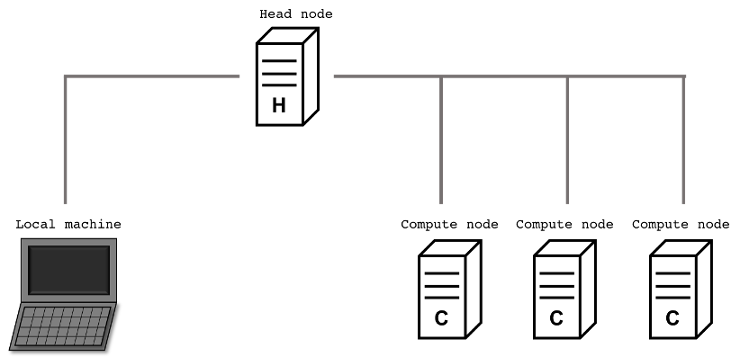
\includegraphics{images/cluster_structure.png}
\caption{Cluster structure}
\end{figure}

    You don't have to log into the head node, you can also log in to a
compute node. When you log into the head node, you can use it to submit
your jobs, migrate data between file systems and housekeeping. However,
you should \textit{\textbf{not}} be running computationally intensive jobs
on the head node outside of LSF.

    \subsection{What is LSF?}\label{what-is-lsf}

When analysing data on a single machine, such as a laptop, commands or
scripts are run in the terminal and the results are given back via the
terminal. On a cluster, we need to run these commands or scripts as
\textbf{jobs}.

The resources required to run the jobs may not always be available
straight away, so the jobs get submitted into a \textbf{queue}. A queue
is a list of jobs which are waiting for resources (pending) or being
executed (running). As jobs in the queue finish executing, the resources
they were using become available again and the next job in the queue
will start running.

Job scheduling and execution is controlled by the platform load sharing
facility (\textbf{LSF}) which manages the workload.

    \begin{figure}[!h]
\centering
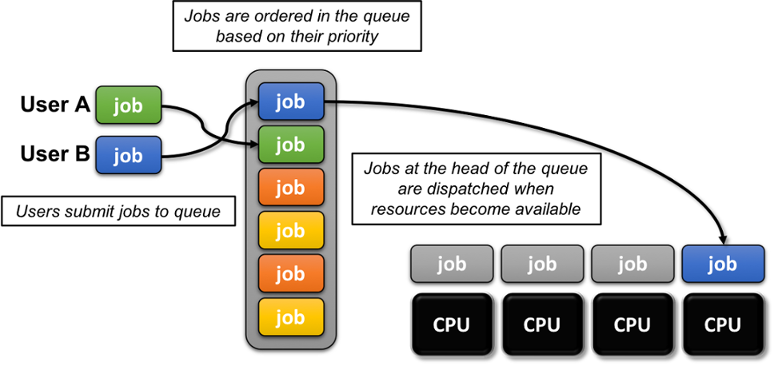
\includegraphics{images/job_processing.png}
\caption{Job processing}
\end{figure}

    For more information, please see the
\href{https://www.ibm.com/support/knowledgecenter/SSETD4_9.1.3/lsf_users_guide/chap_lsf_about.html}{about
LSF} section of the LSF user guide.

    This tutorial assumes that you are currently connected to a cluster
which has LSF installed (e.g. pcs or farm for Sanger users).

\textbf{Let's start by getting some general information about the
cluster.}

\begin{terminalinput}
\begin{Verbatim}[commandchars=\\\{\}]
\llap{\color{black}\LARGE\faKeyboardO\hspace{1em}} lsid
\end{Verbatim}
\end{terminalinput}


    \begin{verbatim}
IBM Platform LSF Standard 9.1.3.0, Jul 04 2014
Copyright IBM Corp. 1992, 2014. All rights reserved.
US Government Users Restricted Rights...

My cluster name is pcs5
My master name is pcs5a
\end{verbatim}

    This should tell you the name of the cluster you're connected to (e.g.
pcs5) and the version of LSF it's using (e.g. 9.1.3.0).

    \textbf{Next, let's take a look at how the cluster is structured.}

\begin{terminalinput}
\begin{Verbatim}[commandchars=\\\{\}]
\llap{\color{black}\LARGE\faKeyboardO\hspace{1em}} lshosts
\end{Verbatim}
\end{terminalinput}


    \begin{verbatim}
HOST_NAME      type    model  cpuf ncpus maxmem maxswp server RESOURCES
pcs5a        X86_64 BL465c_G   8.0    32 255.9G  31.9G    Yes (mg linux lustre)
pcs5b        X86_64 BL465c_G   8.0    32 255.9G  31.9G    Yes (mg linux lustre)
pcs5c        X86_64 BL465c_G   8.0    32 255.9G  31.9G    Yes (linux lustre avx)
pcs5d        X86_64 BL465c_G   8.0    32 255.9G  31.9G    Yes (linux lustre avx)
pcs5e        X86_64 BL465c_G   8.0    32 255.9G  31.9G    Yes (linux lustre avx)
\end{verbatim}

    This should tell you which hosts (nodes) are part of the cluster. In
this example, there are five hosts called pcs5a-e.

\newpage

    \textbf{Finally, let's take get some information about the hosts.}

\begin{terminalinput}
\begin{Verbatim}[commandchars=\\\{\}]
\llap{\color{black}\LARGE\faKeyboardO\hspace{1em}} bhosts
\end{Verbatim}
\end{terminalinput}


    \begin{verbatim}
HOST_NAME          STATUS       JL/U    MAX  NJOBS    RUN  SSUSP  USUSP    RSV
pcs5a              ok              -     16      8      8      0      0      0
pcs5b              ok              -     16      0      0      0      0      0
pcs5c              closed          -     32     32     11      0      0     21
pcs5d              ok              -     32     26     26      0      0      0
pcs5e              ok              -     32     24     20      0      0      4
\end{verbatim}

    For each host, this gives us the host name, host status, job state
statistics, and job slot limits. The host status tells us whether the
host is available and ready to accept new jobs.

There are four possible host status states:

\begin{itemize}
\tightlist
\item
  \textbf{ok} - host is available to accept and run new batch jobs
\item
  \textbf{unavail} - host is down, or load and job management controls
  are unreachable
\item
  \textbf{unreach} - load management controls are running but job
  management controls are unreachable
\item
  \textbf{closed} - host not accepting new jobs
\end{itemize}

To find out why a host is closed you can run \texttt{bhosts} again with
the \texttt{-w} option which returns more detailed information about the
host.

\begin{terminalinput}
\begin{Verbatim}[commandchars=\\\{\}]
\llap{\color{black}\LARGE\faKeyboardO\hspace{1em}} bhosts \PYZhy{}w
\end{Verbatim}
\end{terminalinput}


    \begin{verbatim}
HOST_NAME          STATUS          JL/U    MAX  NJOBS    RUN  SSUSP  USUSP    RSV
pcs5a              ok              -     16      0      0      0      0      0
pcs5b              ok              -     16      0      0      0      0      0
pcs5c              closed_Full     -     32     32     11      0      0     21
pcs5d              ok              -     32     30     26      0      0      4
pcs5e              ok              -     32     28     28      0      0      0
\end{verbatim}

    This tells us that the maximum number of jobs which can be run on that
host has been reached (see values for STATUS, MAX and NJOBS). Once those
jobs have started to complete, the host will be ready to accept new
jobs.

    \begin{center}\rule{0.5\linewidth}{\linethickness}\end{center}

    \subsection{What's next?}\label{whats-next}

For an overview of what this tutorial covers, head to the
\href{index.ipynb}{index}. Otherwise, let's take a closer look at
\href{queues.ipynb}{queues}.


    % Add a bibliography block to the postdoc



\newpage






    \section{Job queues}\label{job-queues}

When you submit a job, the job scheduler will place that job into a
queue. Queues are just lists of submitted jobs which share scheduling
and resource requirements.

    \textbf{To take a look at which queues are available, you can use the
command: \texttt{bqueues}.}

\begin{terminalinput}
\begin{Verbatim}[commandchars=\\\{\}]
\llap{\color{black}\LARGE\faKeyboardO\hspace{1em}} bqueues
\end{Verbatim}
\end{terminalinput}


    \begin{verbatim}
QUEUE_NAME      PRIO STATUS          MAX JL/U JL/P JL/H NJOBS  PEND   RUN  SUSP
system          1000 Open:Active       -    -    -    -     0     0     0     0
yesterday       500  Open:Active      20    8    -    -     0     0     0     0
small            31  Open:Active       -    -    -    -     0     0     0     0
normal           30  Open:Active       -    -    -    -    35    13     1     0
long              3  Open:Active      50    -    -    - 31686 31636    46     0
basement          1  Open:Active      20   10    -    -   180   170    10     0
\end{verbatim}

    This will return information about the queues which are available and
how busy they are. Here, we can see information about six queues into
which jobs can be submitted on the cluster.

By default, \texttt{bqueues} will give you the following information:

    \begin{itemize}
\tightlist
\item
  \textbf{QUEUE\_NAME} - the name of the queue
\item
  \textbf{PRIO} - the priority of the queue
\item
  \textbf{STATUS} - the status of the queue
\item
  \textbf{MAX} - the maximum number of job slots available
\item
  \textbf{JL/U, JL/P and JL/H} - the job slot limit for users,
  processors and hosts respectively
\item
  \textbf{NJOBS} - the total number of tasks for all jobs in the queue
\item
  \textbf{PEND} - the number of pending jobs in the queue
\item
  \textbf{RUN} - the number of running jobs in the queue
\item
  \textbf{SUSP} - the number of suspended jobs in the queue
\end{itemize}

    \begin{center}\rule{0.5\linewidth}{\linethickness}\end{center}

    \subsection{How busy is the cluster?}\label{how-busy-is-the-cluster}

For each queue, you can see the total number of tasks scheduled
(\textbf{NJOBS}) and a breakdown of how many of those jobs are waiting
to be dispatched (\textbf{PEND}), are running (\textbf{RUN}) or are
suspended (\textbf{SUSP}).

    \subsection{Queue priority}\label{queue-priority}

You may have some jobs which are more urgent than others and that you
would like to be run sooner. In these instances, the priority of the
queue is important.

Jobs submitted to higher priority queues are run first. You can check
the queue priority by looking at the \textbf{PRIO} column. The larger
the priority value of the queue, the higher the priority of the queue.
In this example, we can see that the \textbf{yesterday} queue has a much
higher priority than the \textbf{normal} queue and so a job submitted to
the yesterday queue will often be run before a job on the normal queue
if the resources that were requested for that job are available.

For more information on priority and how this works, please see
\href{priority_and_fairshare.ipynb}{priority and fairshare}.

    \subsection{Queue status}\label{queue-status}

Sometimes a queue might not be available. You can check the status of
the queue by looking at the \textbf{STATUS} column.

\begin{itemize}
\tightlist
\item
  \textbf{Open} - the queue \textit{is} able to accept jobs
\item
  \textbf{Closed} - the queue \textit{is not} able to accept jobs
\item
  \textbf{Active} - jobs in the queue will be allowed to start when
  resources are available
\item
  \textbf{Inactive} - jobs in the queue won't be started for the time
  being
\end{itemize}

    \begin{center}\rule{0.5\linewidth}{\linethickness}\end{center}

    \subsection{Getting more information about a particular
queue}\label{getting-more-information-about-a-particular-queue}

You can get more detailed information by using the \texttt{-l} option
with \texttt{bqueues}.

\textbf{Let's try getting some information about the queues on our
cluster.}

\begin{terminalinput}
\begin{Verbatim}[commandchars=\\\{\}]
\llap{\color{black}\LARGE\faKeyboardO\hspace{1em}} bqueues \PYZhy{}l
\end{Verbatim}
\end{terminalinput}


    This will give you the requirements and limits for all of the queues on
the cluster. You can also get the this information for a specific queue
by specifying the name of the queue.

\begin{verbatim}
bqueues -l <queue_name>
\end{verbatim}

In the example command below, we are asking for detailed information
about a queue called yesterday.

    \begin{verbatim}
bqueues -l yesterday
\end{verbatim}

    The \texttt{-l} option will give us a lot more information, such as the
resource limits for the yesterday queue (e.g. maximum memory usage or
run time).

    \begin{verbatim}
QUEUE: yesterday
  -- As in I needed it yesterday highest priority (all nodes)

PARAMETERS/STATISTICS
PRIO NICE STATUS          MAX JL/U JL/P JL/H NJOBS  PEND   RUN SSUSP USUSP  RSV
500   20  Open:Active      20    8    -    -     0     0     0     0     0    0
Interval for a host to accept two jobs is 0 seconds

DEFAULT LIMITS:
 MEMLIMIT
    100 M

MAXIMUM LIMITS:
 RUNLIMIT
     2880.0 min of BL465c_G8

 CORELIMIT MEMLIMIT
      0 M     250 G

SCHEDULING PARAMETERS
           r15s   r1m  r15m   ut      pg    io   ls    it    tmp    swp    mem
 loadSched   -     -     -     -       -     -    -     -     -      -      -
 loadStop    -     -     -     -       -     -    -     -     -      -      -

              poe nrt_windows adapter_windows ntbl_windows  uptime
 loadSched     -           -               -            -       -
 loadStop      -           -               -            -       -

SCHEDULING POLICIES:  FAIRSHARE
USER_SHARES:  [default, 1]

SHARE_INFO_FOR: yesterday/
USER/GROUP   SHARES  PRIORITY  STARTED  RESERVED  CPU_TIME  RUN_TIME   ADJUST
user1            1       0.302      0        0        47.0     1590       0.000
user2            1       0.301      0        0       590.3     1634       0.000

USERS: all
HOSTS:  pcs5a pcs5b+1 others+2
RES_REQ:  select[type==any]
Maximum slot reservation time: 14400 seconds
\end{verbatim}

    Below is an example for three queues which have different resource
limits. Here, jobs in the normal queue will automatically be terminated
or killed by LSF if they try to run for more than 12 hours (RUNLIMIT =
720.0 min), in the long queue after 2 days (RUNLIMIT = 2880.0 min) and
in the hugemem queue after 15 days (RUNLIMIT = 21600.0 min). The hugemem
also has a much larger memory limit (727.5G) than the normal or long
queues (250G).

    \textbf{normal}:

\begin{verbatim}
 RUNLIMIT
 720.0 min of BL465c_G8

 CORELIMIT MEMLIMIT
      0 M     250 G
\end{verbatim}

\textbf{long}:

\begin{verbatim}
 RUNLIMIT
 2880.0 min of BL465c_G8

 CORELIMIT MEMLIMIT
      0 M     250 G
\end{verbatim}

\textbf{hugemem}:

\begin{verbatim}
 RUNLIMIT
 21600.0 min of HS21_E5450_8

 CORELIMIT MEMLIMIT
      0 M   727.5 G
\end{verbatim}

    For more information, please see the
\href{https://www.ibm.com/support/knowledgecenter/SSETD4_9.1.3/lsf_admin/chap_queues_working_with.html}{working
with queues} section of the LSF user guide.

    \begin{center}\rule{0.5\linewidth}{\linethickness}\end{center}

    \subsection{What's next?}\label{whats-next}

For an overview of the key concepts, you can go back to the
\href{index.ipynb}{introduction}. Otherwise, let's take a look at
\href{submitting_jobs.ipynb}{submitting jobs}.


    % Add a bibliography block to the postdoc



\newpage






    \section{Submitting jobs}\label{submitting-jobs}

When analysing data on a single machine, such as a laptop, commands or
scripts are run in the terminal and the results are given back to us in
that terminal. For example, the \texttt{sleep} command tells your
machine to suspend the execution of a command for a defined period of
time (in seconds).

\textbf{Let's tell our machine to pause for 60 seconds.}

\begin{terminalinput}
\begin{Verbatim}[commandchars=\\\{\}]
\llap{\color{black}\LARGE\faKeyboardO\hspace{1em}} sleep 60
\end{Verbatim}
\end{terminalinput}


    When using a cluster, these commands or scripts need to be submitted as
jobs. To submit a job with LSF, we use the \texttt{bsub} command.

\textbf{Now, let's submit the previous command as a job using
\texttt{bsub}.}

\begin{terminalinput}
\begin{Verbatim}[commandchars=\\\{\}]
\llap{\color{black}\LARGE\faKeyboardO\hspace{1em}} bsub \PY{l+s+s2}{\PYZdq{}sleep 60\PYZdq{}}
\end{Verbatim}
\end{terminalinput}


    \begin{verbatim}
Returning output by mail is not supported on this cluster.
Please use the -o option to write output to disk.
Job <4015755> is submitted to default queue <normal>.
\end{verbatim}

    When you submit a job, it will be given a unique identifier (e.g.
4015755) which will help us with getting updates on what's happening
with our job. To find out what jobs are scheduled and running, we can
use another command, \texttt{bjobs}.

\textbf{We can see how our job is getting on by running \texttt{bjobs}.}

\begin{terminalinput}
\begin{Verbatim}[commandchars=\\\{\}]
\llap{\color{black}\LARGE\faKeyboardO\hspace{1em}} bjobs
\end{Verbatim}
\end{terminalinput}


    \begin{verbatim}
JOBID   USER    STAT  QUEUE      FROM_HOST   EXEC_HOST   JOB_NAME   SUBMIT_TIME
4015755 abc     PEND  normal     pcs5b                   sleep 10   Jan 15 14:06
\end{verbatim}

    This will give us the following information:

\begin{itemize}
\tightlist
\item
  \textbf{JOBID} - unique numerical job identifier used to keep track of
  the job
\item
  \textbf{USER} - username of the person who submitted the job
\item
  \textbf{STAT} - job state
\item
  \textbf{QUEUE} - which queue the job was submitted to
\item
  \textbf{FROM\_HOST} - which host the job was submitted from
\item
  \textbf{EXEC\_HOST} - which host the job is running on (blank if job
  is pending)
\item
  \textbf{JOB\_NAME} - name of the job
\item
  \textbf{SUBMIT\_TIME} - when the job was submitted
\end{itemize}

    Most jobs will have one of three states (STAT):

\begin{itemize}
\tightlist
\item
  \textbf{PEND} - the job is waiting in the queue to be scheduled and
  dispatched
\item
  \textbf{RUN} - the job has been dispatched to a host (node) and is
  running
\item
  \textbf{DONE} - the jobs finished normally (has an exit value of 0)
\end{itemize}

\newpage

Occasionally, you may also see suspended job states:

\begin{itemize}
\tightlist
\item
  \textbf{PSUSP} - job was suspended by the owner or administrator while
  pending
\item
  \textbf{USUSP} - job was suspended by the owner or administrator after
  being dispatched
\item
  \textbf{SSUSP} - job was suspended by LSF after being dispatched
\end{itemize}

    In this example, we can see that our job was submitted to the
\textit{normal} queue by default and that it hasn't started yet
(\textit{PEND}).

\textbf{Let's check again.}

\begin{terminalinput}
\begin{Verbatim}[commandchars=\\\{\}]
\llap{\color{black}\LARGE\faKeyboardO\hspace{1em}} bjobs
\end{Verbatim}
\end{terminalinput}


    \begin{verbatim}
JOBID   USER    STAT  QUEUE      FROM_HOST   EXEC_HOST   JOB_NAME   SUBMIT_TIME
4015755 abc     RUN   normal     pcs5b       pcs5c       sleep 10   Jan 15 14:06
\end{verbatim}

    Here we can see that our job has now started running (\textit{RUN}) and is
being executed on \textit{pcs5c} (EXEC\_HOST).

\textbf{Let's wait a little longer and check one more time.}

\begin{terminalinput}
\begin{Verbatim}[commandchars=\\\{\}]
\llap{\color{black}\LARGE\faKeyboardO\hspace{1em}} bjobs
\end{Verbatim}
\end{terminalinput}


    \begin{verbatim}
No unfinished job found
\end{verbatim}

    Now we can't see any jobs. Why? That's because our job has finished
running and we have no more jobs scheduled.

Did you notice the message that was returned when you submitted your
job?

    \begin{verbatim}
Returning output by mail is not supported on this cluster.
Please use the -o option to write output to disk.
\end{verbatim}

    This is because we used the default options and didn't specify an output
file or an error file. We'll be looking at why printing the job outputs
to files is good practice (and very useful!) in the next section.

You can find more information on job submission in general by looking
through the
\href{https://www.ibm.com/support/knowledgecenter/SSETD4_9.1.3/lsf_users_guide/job_submit.html}{job
submission} and
\href{https://www.ibm.com/support/knowledgecenter/SSETD4_9.1.3/lsf_admin/job_info_view_lsf.html}{job
information} sections of the LSF user manual.

    \begin{center}\rule{0.5\linewidth}{\linethickness}\end{center}

    \subsection{What's next?}\label{whats-next}

For another look at queues, you can go back to
\href{queues.ipynb}{queues}. Otherwise, let's take a closer look at
\href{managing_jobs.ipynb}{managing jobs}.


    % Add a bibliography block to the postdoc



\newpage






    \section{Managing jobs}\label{managing-jobs}

    In this section, we'll be taking a closer look at submitting jobs and
how you can manage them once they've been submitted.

    \subsection{Writing job outputs to
file}\label{writing-job-outputs-to-file}

In the previous section, we looked at submitting a job using the default
options using \texttt{bsub}.

\begin{terminalinput}
\begin{Verbatim}[commandchars=\\\{\}]
\llap{\color{black}\LARGE\faKeyboardO\hspace{1em}} bsub \PY{l+s+s2}{\PYZdq{}sleep 60\PYZdq{}}
\end{Verbatim}
\end{terminalinput}


    That submission returned a message:

    \begin{verbatim}
Returning output by mail is not supported on this cluster.
Please use the -o option to write output to disk.
\end{verbatim}

    This message is saying that no matter whether the job succeeds or fails,
we don't know what resources it used or if there were any errors because
we didn't store that information anywhere. Not tracking information
about your job and the outputs and errors it produces makes it difficult
to troubleshoot any issues with the job execution.

What we can do instead is supply an output file using the \texttt{-o}
option and an error file using the \texttt{-e} option.

    \begin{verbatim}
bsub -o <output_file> -e <error_file> "command"
\end{verbatim}

    \textbf{Let's give this a try. We'll call our output and error files
\textit{myjob.o} and \textit{myjob.e}.}

\begin{terminalinput}
\begin{Verbatim}[commandchars=\\\{\}]
\llap{\color{black}\LARGE\faKeyboardO\hspace{1em}} bsub \PYZhy{}o myjob.o \PYZhy{}e myjob.e \PY{l+s+s2}{\PYZdq{}sleep 60\PYZdq{}}
\end{Verbatim}
\end{terminalinput}


    \textbf{You can check the progress of your job using \texttt{bjobs}.}

\begin{terminalinput}
\begin{Verbatim}[commandchars=\\\{\}]
\llap{\color{black}\LARGE\faKeyboardO\hspace{1em}} bjobs
\end{Verbatim}
\end{terminalinput}


    \textbf{When the job has finished, print the contents of the output file
to terminal using \texttt{cat}.}

\begin{terminalinput}
\begin{Verbatim}[commandchars=\\\{\}]
\llap{\color{black}\LARGE\faKeyboardO\hspace{1em}} cat myjob.o
\end{Verbatim}
\end{terminalinput}


    \begin{verbatim}
------------------------------------------------------------
Sender: LSF System <lsfadmin@pcs5a>
Subject: Job 4018040: <sleep 60> in cluster <pcs5> Done

Job <sleep 60> was submitted from host <pcs5a> by user <userA> in cluster <pcs5>.
Job was executed on host(s) <pcs5a>, queue <normal>, user <userA> cluster <pcs5>.
</nfs/users/nfs_u/userA> was used as the home directory.
</nfs/users/nfs_u/userA> was used as the working directory.
Started at Thu Jan 15 12:26:45 2019
Results reported on Thu Jan 15 12:27:45 2019

Your job looked like:

------------------------------------------------------------
# LSBATCH: User input
sleep 60
------------------------------------------------------------

Successfully completed.

Resource usage summary:

    CPU time :                                   0.82 sec.
    Max Memory :                                 5 MB
    Average Memory :                             5.00 MB
    Total Requested Memory :                     -
    Delta Memory :                               -
    Max Swap :                                   44 MB
    Max Processes :                              3
    Max Threads :                                4

The output (if any) is above this job summary.



PS:

Read file <myjob.e> for stderr output of this job.
\end{verbatim}

    \textbf{Now, look at your error file using \texttt{cat}.}

\begin{terminalinput}
\begin{Verbatim}[commandchars=\\\{\}]
\llap{\color{black}\LARGE\faKeyboardO\hspace{1em}} cat myjob.e
\end{Verbatim}
\end{terminalinput}


    Printing our error file won't return anything as the error file was
empty. This is because our job didn't have any errors. If it did, they
would be logged in the error file and we could use it to try and trace
what went wrong.

    You can also incorporate your JOBID into the filename using a special
variable \textbf{\%J}.

    \begin{verbatim}
bsub -o %J.o -e %J.e "sleep 60"
\end{verbatim}

    Let's say that the JOBID returned when you submitted the job was
4018041. Your output and error files would be called \textit{4018041.o}
and \textit{4018041.e}.

You should always try to have different output and error files for each
job your submitting. If you submit two jobs writing to \textit{myjob.o}
and \textit{myjob.e} then it can get confusing as they are both writing to
the same file.

    \subsection{Giving your job a name}\label{giving-your-job-a-name}

You may have noticed that when you submitted your job earlier and
checked its progress with \texttt{bjobs} that the JOB\_NAME was
\textit{sleep 60}. This is because, by default, if no job name is given
when you submit the job, the job name will become the command that you
submitted.

    \begin{verbatim}
JOBID   USER    STAT  QUEUE      FROM_HOST   EXEC_HOST   JOB_NAME   SUBMIT_TIME
4018040 UserA   PEND  normal     pcs5a       pcs5b       sleep 60   Jan 15 13:26
\end{verbatim}

    You can give your job a different name using the \texttt{-J} option with
\texttt{bsub}. This can be useful when you're running multiple jobs and
want to be able to tell them apart in the queue with \texttt{bjobs}.

\textbf{Let's try submitting a job called "newjob" which writes outputs
and errors to \textit{newjob.o} and \textit{newjob.e}.}

\begin{terminalinput}
\begin{Verbatim}[commandchars=\\\{\}]
\llap{\color{black}\LARGE\faKeyboardO\hspace{1em}} bsub \PYZhy{}o newjob.o \PYZhy{}e newjob.e \PYZhy{}J newjob \PY{l+s+s2}{\PYZdq{}sleep 60\PYZdq{}}
\end{Verbatim}
\end{terminalinput}


    \textbf{Let's look at the progress of our job using \texttt{bjobs}.}

\begin{terminalinput}
\begin{Verbatim}[commandchars=\\\{\}]
\llap{\color{black}\LARGE\faKeyboardO\hspace{1em}} bjobs
\end{Verbatim}
\end{terminalinput}


    \begin{verbatim}
JOBID   USER    STAT  QUEUE      FROM_HOST   EXEC_HOST   JOB_NAME   SUBMIT_TIME
4018077 UserA   RUN   normal     pcs5a       pcs5b       newjob     Jan 15 13:34
\end{verbatim}

    Notice that the JOB\_NAME is now \textit{newjob}.

    \begin{center}\rule{0.5\linewidth}{\linethickness}\end{center}

    \subsection{Submitting your job to a particular
queue}\label{submitting-your-job-to-a-particular-queue}

If we don't specify a queue when we submit a job, the job will be
submitted to the default queue. To find out which one of the queues is
used by default, we can use the command \texttt{bparams}.

\begin{terminalinput}
\begin{Verbatim}[commandchars=\\\{\}]
\llap{\color{black}\LARGE\faKeyboardO\hspace{1em}} bparams
\end{Verbatim}
\end{terminalinput}


    \begin{verbatim}
Default Queues:  normal
Default Host Specification:  BL465c_G8
MBD_SLEEP_TIME used for calculations:  10 seconds
Job Checking Interval:  15 seconds
Job Accepting Interval:  0 seconds
\end{verbatim}

    Running \texttt{bparams} will display information about the system
parameters, such as the default queue name. In this example, the default
queue is the \textit{normal} queue. To find out which other queues are
available, we can use \texttt{bqueues}.

\begin{terminalinput}
\begin{Verbatim}[commandchars=\\\{\}]
\llap{\color{black}\LARGE\faKeyboardO\hspace{1em}} bqueues
\end{Verbatim}
\end{terminalinput}

\newpage

    \begin{verbatim}
QUEUE_NAME      PRIO STATUS          MAX JL/U JL/P JL/H NJOBS  PEND   RUN  SUSP
system          1000 Open:Active       -    -    -    -     0     0     0     0
yesterday       500  Open:Active      20    8    -    -     0     0     0     0
small            31  Open:Active       -    -    -    -     0     0     0     0
normal           30  Open:Active       -    -    -    -   103    43    60     0
long              3  Open:Active      50    -    -    -   241   224    15     0
basement          1  Open:Active      20   10    -    -   182   164    18     0
\end{verbatim}

    Now, let's say that we want to submit a job into the \textit{yesterday}
queue because it's fairly urgent. To do this, we can use the \texttt{-q}
option with \texttt{bsub} followed by the name of the queue which we
want to use (e.g. \textit{yesterday}).

\textbf{Let's try submitting a job into the yesterday queue called
"newjob1" which writes outputs and errors to newjob1.o and newjob1.e.}

\begin{terminalinput}
\begin{Verbatim}[commandchars=\\\{\}]
\llap{\color{black}\LARGE\faKeyboardO\hspace{1em}} bsub \PYZhy{}o newjob1.o \PYZhy{}e newjob1.e \PYZhy{}J newjob1 \PYZhy{}q yesterday \PY{l+s+s2}{\PYZdq{}sleep 60\PYZdq{}}
\end{Verbatim}
\end{terminalinput}


    When you check on the progress with \texttt{bjobs} you will see that job
is in the \textit{yesterday} queue.

    \begin{verbatim}
JOBID   USER    STAT  QUEUE      FROM_HOST   EXEC_HOST   JOB_NAME   SUBMIT_TIME
4018119 UserA   RUN   yesterday  pcs5a       pcs5c       newjob1    Jan 15 13:51
\end{verbatim}

    \begin{center}\rule{0.5\linewidth}{\linethickness}\end{center}

    \subsection{Job resources}\label{job-resources}

When we want to reserve more resources for our jobs, we can use the
\texttt{-R}, \texttt{-M} and \texttt{-n} options with the \texttt{bsub}
command. The \texttt{-M} option sets LSF the memory limit, \texttt{-n}
sets the thread limit and the \texttt{-R} option tells LSF that the job
needs to run on a host which matches the requirements which follow it.

\textbf{Let's try submitting a job which has a limit of 2GB memory and 4
threads.}

\begin{terminalinput}
\begin{Verbatim}[commandchars=\\\{\}]
\llap{\color{black}\LARGE\faKeyboardO\hspace{1em}} bsub \PYZhy{}n \PY{l+m}{4} \PYZhy{}R \PY{l+s+s2}{\PYZdq{}span[hosts=1] select[mem\PYZgt{}2000] rusage[mem=2000]\PYZdq{}} \PY{l+s+se}{\PYZbs{}}
        \PYZhy{}M \PY{l+m}{2000} \PY{l+s+s2}{\PYZdq{}sleep 60\PYZdq{}}
\end{Verbatim}
\end{terminalinput}


    Here we can see that the 4 threads are reserved using the \texttt{-n}
option. Typically when we ask for multiple threads with \texttt{-n}, we
also add \textbf{span{[}hosts=1{]}} to the \texttt{-R} option. This
indicates that all the processors which are allocated to this job must
be on the same host.

We reserve our 2GB of memory using the \texttt{-M} options and
\texttt{-R} option. Notice that the memory requirement is given in MB
(2GB \textasciitilde{} 2000MB). With the \texttt{-R} option, we use a
select string, \textbf{select{[}mem\textgreater{}2000{]}}, and a usage
string, \textbf{rusage{[}mem=2000{]}}. The selection string specifies
the characteristics that a host must have to match the resource
requirement. In this case, more than 2GB memory. The usage string
defines the expected resource usage of the job. By default, no resources
are reserved.

For more information on resource requirements, please see the
\href{https://www.ibm.com/support/knowledgecenter/SSETD4_9.1.3/lsf_admin/res_req_strings_about.html}{resource
requirement} section of the LSF user manual.


    \subsection{Job workflow}\label{job-workflow}

Once you have submitted your job, there are several different ways in
which you can manage it. Below is a diagram which shows the typical job
workflows and related commands.

    \begin{figure}[!h]
\centering
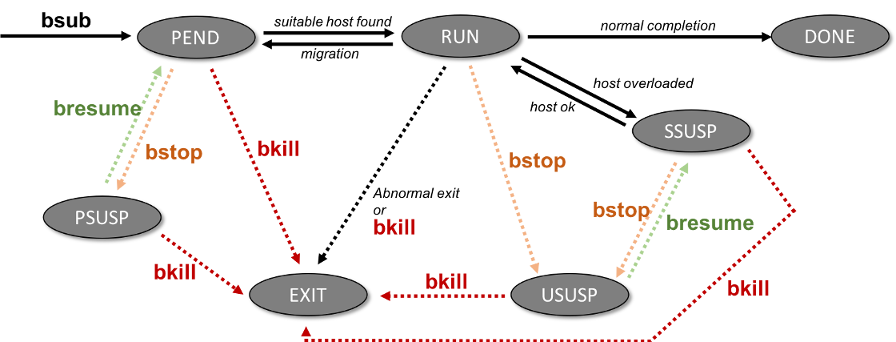
\includegraphics{images/lsf_workflow.png}
\caption{LSF job workflow}
\end{figure}

    Along the top of the diagram is the simplest job workflow. Here, a job
is submitted using \texttt{bsub} and will have the status \textit{PEND}
until it gets dispatched.

    \begin{verbatim}
JOBID   USER    STAT  QUEUE      FROM_HOST   EXEC_HOST   JOB_NAME   SUBMIT_TIME
1000    userA   PEND  normal     pcs5b                   job1       Jan 15 14:06
\end{verbatim}

    Once the job is dispatched, it will start running and get the status
\textit{RUN}.

    \begin{verbatim}
JOBID   USER    STAT  QUEUE      FROM_HOST   EXEC_HOST   JOB_NAME   SUBMIT_TIME
1000    userA   RUN   normal     pcs5b       pcs5c       job1       Jan 15 14:06
\end{verbatim}

    If all goes well and there are no errors (normal completion) then the
job finishes and has the status \textit{DONE}.

    \begin{verbatim}
JOBID   USER    STAT  QUEUE      FROM_HOST   EXEC_HOST   JOB_NAME   SUBMIT_TIME
1000    userA   DONE  normal     pcs5b       pcs5c       job1       Jan 15 14:06
\end{verbatim}

    If there is a problem with a running job, this will trigger an abnormal
exit and the status will become \textit{EXIT}.

    \begin{verbatim}
JOBID   USER    STAT  QUEUE      FROM_HOST   EXEC_HOST   JOB_NAME   SUBMIT_TIME
1000    userA   EXIT  normal     pcs5b       pcs5c       job1       Jan 15 14:06
\end{verbatim}

    \subsubsection{Cancelling jobs}\label{cancelling-jobs}

Now, let's consider some deviations from this workflow. First, how do we
cancel a job once it's been submitted?

    \begin{verbatim}
JOBID   USER    STAT  QUEUE      FROM_HOST   EXEC_HOST   JOB_NAME   SUBMIT_TIME
1000    userA   PEND  normal     pcs5b                   job1       Jan 15 14:06
\end{verbatim}

    We can cancel or kill a job 1000 using the command \texttt{bkill}
followed by the JOBID of the job that you want to kill.

    \begin{verbatim}
bkill 1000
\end{verbatim}

    If you have used a valid JOBID, the \texttt{bkill} command should return
a message that tells you the job is being terminated.

    \begin{verbatim}
Job <1000> is being terminated
\end{verbatim}

    Your job status will now get updated from \textit{RUN} or \textit{PEND} to
\textit{EXIT}.

    \begin{verbatim}
JOBID   USER    STAT  QUEUE      FROM_HOST   EXEC_HOST   JOB_NAME   SUBMIT_TIME
1000    userA   EXIT  normal     pcs5b                   job1       Jan 15 14:06
\end{verbatim}

    \subsubsection{Suspending and resuming
jobs}\label{suspending-and-resuming-jobs}

Let's say you are running a series of commands and you realise there's
an error in the input file for one of those commands. When you're
running a long job, you probably don't want to have to cancel it and
start all over again. If the job hasn't reached that command, you can
pause or suspend the job while you fix the input file and resume the job
once you're done.

To suspend and resume a job you can use the \texttt{bstop} and
\texttt{bresume} commands. First let's look at suspending a pending job
(\textit{PEND}).

\begin{verbatim}
JOBID   USER    STAT  QUEUE      FROM_HOST   EXEC_HOST   JOB_NAME   SUBMIT_TIME
1000    userA   PEND  normal     pcs5b                   job1       Jan 15 14:06
\end{verbatim}

    To suspend this job, we use \texttt{bstop} followed by the JOBID.

    \begin{verbatim}
bstop 1000
\end{verbatim}

    The job status will now become \textit{PSUSP} as the job was suspended by
a user while it was pending.

    \begin{verbatim}
JOBID   USER    STAT  QUEUE      FROM_HOST   EXEC_HOST   JOB_NAME   SUBMIT_TIME
1000    userA   PSUSP normal     pcs5b                   job1       Jan 15 14:06
\end{verbatim}

    To allow the job to be dispatched again, we can use the command
\texttt{bresume} followed by the JOBID.

    \begin{verbatim}
bresume 1000
\end{verbatim}

    The job status will now return back to \textit{PEND} while the job waits
to be dispatched.

    \begin{verbatim}
JOBID   USER    STAT  QUEUE      FROM_HOST   EXEC_HOST   JOB_NAME   SUBMIT_TIME
1000    userA   PEND  normal     pcs5b                   job1       Jan 15 14:06
\end{verbatim}

    You can also suspend a running job using \texttt{bstop}. In this case,
the status will be updated to \textit{USUSP} instead of \textit{PSUSP}.

    \begin{verbatim}
JOBID   USER    STAT  QUEUE      FROM_HOST   EXEC_HOST   JOB_NAME   SUBMIT_TIME
1000    userA   USUSP normal     pcs5b                   job1       Jan 15 14:06
\end{verbatim}

    When you resume a previously running job that has been suspended with
\texttt{bresume}, there may be an interim status of \textit{SSUSP} before
the job starts running again (\textit{RUN}).

For more information on suspending, resuming and cancelling jobs, please
see the
\href{https://www.ibm.com/support/knowledgecenter/en/SSWRJV_10.1.0/lsf_admin_foundations/control_job_exec.html}{controlling
job execution} section in the LSF user guide.

    \subsection{Moving a job to a different
queue}\label{moving-a-job-to-a-different-queue}

Let's use as an example, a job which has been submitted to the
\textit{normal} queue and is waiting to be dispatched (PEND).

    \begin{verbatim}
JOBID   USER    STAT  QUEUE      FROM_HOST   EXEC_HOST   JOB_NAME   SUBMIT_TIME
1000    userA   PEND  normal     pcs5b                   job1       Jan 15 14:06
\end{verbatim}

    Now, let's say that we've made a mistake and that we know this submitted
job will run for longer than the \textit{normal} queue will allow. What
can we do?

Well, you could kill the job with \texttt{bkill} followed by the JOBID
of the job you want to cancel. You can then submit the job again
specifying a different queue using the \texttt{bsub} option \texttt{-q}
and the name of the queue you want to use. This would create a new job
in a different queue (e.g. \textit{long}).

    \begin{verbatim}
bkill <JOBID>
bsub -q <queue_name> <command>
\end{verbatim}

    Alternatively, you can move the pending job to a different queue using
\texttt{bswitch}.

    \begin{verbatim}
bswitch <destination_queue> <JOBID>
\end{verbatim}

    So, to move our job (JOBID = 1000) from the \textit{normal} queue (jobs
killed after 12 hours) to the \textit{long} queue (jobs killed after 48
hours) we would run:

    \begin{verbatim}
bswitch long 1000
\end{verbatim}

    And if we looked again using \texttt{bjobs} we can see that the job has
been moved into the \texttt{long} queue.

    \begin{verbatim}
JOBID   USER    STAT  QUEUE      FROM_HOST   EXEC_HOST   JOB_NAME   SUBMIT_TIME
1000    userA   PEND  long       pcs5b                   job1       Jan 15 14:06
\end{verbatim}

    For more information on moving jobs between queues, please see the
\href{https://www.ibm.com/support/knowledgecenter/SSETD4_9.1.3/lsf_admin/job_switch_queue.html}{switching
queues} section of the LSF user guide.

    \begin{center}\rule{0.5\linewidth}{\linethickness}\end{center}

    \subsection{What's next?}\label{whats-next}

For an overview of basic job submission, you can go back to
\href{job_submission.ipynb}{job submission}. Otherwise, let's take a
look at \href{job_arrays.ipynb}{job arrays and dependencies}.


    % Add a bibliography block to the postdoc



\newpage






    \section{Job arrays and dependencies}\label{job-arrays-and-dependencies}

    In this section, we're going to take a look at how to submit a script
instead of a command. We'll then use a script to help us submit a large
number of identical tasks as a single job with a single JOBID. Finally,
we'll take a look at how to submit a job that's dependent on another
job.


    \subsection{Writing and submitting
scripts}\label{writing-and-submitting-scripts}

    Earlier on, we were submitting a single command as a job.

\textbf{Let's run that \texttt{bsub} command again.}

\begin{terminalinput}
\begin{Verbatim}[commandchars=\\\{\}]
\llap{\color{black}\LARGE\faKeyboardO\hspace{1em}} bsub \PY{l+s+s2}{\PYZdq{}sleep 60\PYZdq{}}
\end{Verbatim}
\end{terminalinput}


    But, what if want wanted to submit several commands in a single job? For
this, we can use a shell script. We can write a series of commands in a
file (our script) which will read in a DNA sequence and substitutes the
letters/bases to return the complimentary sequence (A -\textgreater{} T,
T -\textgreater{} A, C -\textgreater{} G and G -\textgreater{} C).

Here, we've written the into a file called \texttt{myscript.sh}. We can
use \texttt{cat} to print the contents of our script
\texttt{myscript.sh} to the terminal.

\textbf{Use \texttt{cat} to see the contents of \textit{myscript.sh}.}

\begin{terminalinput}
\begin{Verbatim}[commandchars=\\\{\}]
\llap{\color{black}\LARGE\faKeyboardO\hspace{1em}} cat myscript.sh
\end{Verbatim}
\end{terminalinput}


    Notice that at the top we've added the line "\#!/bin/bash" which tells
the system the script should always be run with bash, rather than
another shell.

    \begin{verbatim}
#!/bin/bash

input=$(<data/sequence.txt)
echo "Input sequence: $input"

output=$(echo $input | tr 'ATGC' 'TACG')
echo "Complementary sequence: $output"
\end{verbatim}

    There's one thing that we need to do before submitting our script.
Before we can submit our script, we need to make sure the system
recognises our file as a script. We can do this using \texttt{chmod} to
make our script executable.

\textbf{Make \textit{myscript.sh} executable.}

\begin{terminalinput}
\begin{Verbatim}[commandchars=\\\{\}]
\llap{\color{black}\LARGE\faKeyboardO\hspace{1em}} chmod u+x myscript.sh
\end{Verbatim}
\end{terminalinput}



    \textbf{Try running \textit{myscript.sh} directly in the terminal.}

\begin{terminalinput}
\begin{Verbatim}[commandchars=\\\{\}]
\llap{\color{black}\LARGE\faKeyboardO\hspace{1em}} ./myscript.sh
\end{Verbatim}
\end{terminalinput}

\newpage

    In your terminal there should now be a message with the original
sequence, read from an input file by the script, and the corresponding
complementary sequence.

    \begin{verbatim}
Input sequence: AAAGGTTC
Complementary sequence: TTTCCAAG
\end{verbatim}

    \textbf{To submit this script as a job, use \texttt{bsub}.}

\begin{terminalinput}
\begin{Verbatim}[commandchars=\\\{\}]
\llap{\color{black}\LARGE\faKeyboardO\hspace{1em}} bsub \PYZhy{}o myscript.o \PYZhy{}e myscript.e \PY{l+s+s2}{\PYZdq{}./myscript.sh\PYZdq{}}
\end{Verbatim}
\end{terminalinput}


    \textbf{Check the status of your job using \texttt{bjobs}.}

\begin{terminalinput}
\begin{Verbatim}[commandchars=\\\{\}]
\llap{\color{black}\LARGE\faKeyboardO\hspace{1em}} bjobs
\end{Verbatim}
\end{terminalinput}


    \textbf{Once the job has finished, take a look at the output file which
was generated.}

\begin{terminalinput}
\begin{Verbatim}[commandchars=\\\{\}]
\llap{\color{black}\LARGE\faKeyboardO\hspace{1em}} cat myscript.o
\end{Verbatim}
\end{terminalinput}


    At the top you should see the input and complementary sequences which
means that your script executed as we'd expect.

    \begin{verbatim}
Input sequence: AAAGGTTC
Complementary sequence: TTTCCAAG

------------------------------------------------------------
Sender: LSF System <lsfadmin@pcs5e>
Subject: Job 4019973: <./myscript.sh> in cluster <pcs5> Done

...
\end{verbatim}

    \begin{center}\rule{0.5\linewidth}{\linethickness}\end{center}

    \subsection{Submitting an array of
jobs}\label{submitting-an-array-of-jobs}

    Sometimes, you may want to run the same commands across lots of files.
This is common in pipelines where your jobs will be identical except for
the input data they are working on.

For example, let's say we want to find complementary sequences from in 5
different sequence files. We've named these sequence files so that a
number from 1 to 5 is the suffix(sequence.txt.{[}1-5{]}).

\textbf{Take a look at the files in the data directory using
\texttt{ls}.}

\begin{terminalinput}
\begin{Verbatim}[commandchars=\\\{\}]
\llap{\color{black}\LARGE\faKeyboardO\hspace{1em}} ls data
\end{Verbatim}
\end{terminalinput}



    You should see files called \textit{sequence.txt} followed by a number
between 1 and 5.

    \begin{verbatim}
sequence.txt    sequence.txt.2  sequence.txt.4
sequence.txt.1  sequence.txt.3  sequence.txt.5
\end{verbatim}

\newpage

    We've provided a second script, \textit{myarrayscript.sh}, which is almost
the same as \textit{myscript.sh} except that it includes an environment
variable, \textbf{\$LSB\_JOBINDEX}, to tell the script which file to use
as input.

\textbf{Look at contents of \textit{myarrayscript.sh} using \texttt{cat}.}

\begin{terminalinput}
\begin{Verbatim}[commandchars=\\\{\}]
\llap{\color{black}\LARGE\faKeyboardO\hspace{1em}} cat myarrayscript.sh
\end{Verbatim}
\end{terminalinput}


    Here, we can see the use of \textbf{\$LSB\_JOBINDEX} at the end of the
input filename (infile). As LSF iterates through the job array, this
number will increase so that the first job in the array will read in
\textit{sequence.txt.1} and the second job, \_sequence.txt.2 ... and so
on.

    \begin{verbatim}
#!/bin/bash

infile=data/sequence.txt.$LSB_JOBINDEX
echo "Reading $infile"

input=$(<$infile)
echo "Input sequence: $input"

output=$(echo $input | tr 'ATGC' 'TACG')
echo "Complementary sequence: $output"

echo "Done"
\end{verbatim}

    \textbf{Don't forget to update the permissions on the script so that we
can use it.}

\begin{terminalinput}
\begin{Verbatim}[commandchars=\\\{\}]
\llap{\color{black}\LARGE\faKeyboardO\hspace{1em}} chmod u+x myarrayscript.sh
\end{Verbatim}
\end{terminalinput}


    The submission command below uses two special variables, \textbf{\%J}
and \textbf{\%I}, in the output file names which represent the JOBID and
the JOBINDEX. The JOBID will be the same for all of the jobs in this
array and the JOBINDEX, which identifies which job was run from the
array, will correspond to the number at the end of our filenames
(\$LSF\_JOBINDEX).

\textbf{Let's submit our job array.}

\begin{terminalinput}
\begin{Verbatim}[commandchars=\\\{\}]
\llap{\color{black}\LARGE\faKeyboardO\hspace{1em}} bsub \PYZhy{}J\PY{l+s+s2}{\PYZdq{}sequence[1\PYZhy{}5]\PYZdq{}} \PYZhy{}o sequence.out.\PYZpc{}J\PYZhy{}\PYZpc{}I ./myarrayscript.sh
\end{Verbatim}
\end{terminalinput}


    \textbf{Check the progress of the jobs.}

\begin{terminalinput}
\begin{Verbatim}[commandchars=\\\{\}]
\llap{\color{black}\LARGE\faKeyboardO\hspace{1em}} bjobs
\end{Verbatim}
\end{terminalinput}


    When you check on the progress using \texttt{bjobs} you will see five
jobs running. Here is an example output from \texttt{bjobs}.

    \begin{verbatim}
JOBID   USER    STAT  QUEUE      FROM_HOST   EXEC_HOST   JOB_NAME   SUBMIT_TIME
4019986 userA   RUN   normal     pcs5a       pcs5e       *quence[1] Jan 15 13:46
4019986 userA   RUN   normal     pcs5a       pcs5e       *quence[2] Jan 15 13:46
4019986 userA   RUN   normal     pcs5a       pcs5e       *quence[3] Jan 15 13:46
4019986 userA   RUN   normal     pcs5a       pcs5e       *quence[4] Jan 15 13:46
4019986 userA   RUN   normal     pcs5a       pcs5e       *quence[5] Jan 15 13:46
\end{verbatim}

    Notice here that there are five jobs, one for each of our input files,
and that the JOBID is the same for all of the jobs (4019986). If we look
at the JOB\_NAME, LSF has added the JOBINDEX to the end of each of the
job names (e.g. {[}1{]}).

\textbf{Once your jobs have finished you can look for the output files
using \texttt{ls}.}

\begin{terminalinput}
\begin{Verbatim}[commandchars=\\\{\}]
\llap{\color{black}\LARGE\faKeyboardO\hspace{1em}} ls sequence.out*
\end{Verbatim}
\end{terminalinput}


    You should see five files. Each of the filenames will begin with
\textit{sequence.out}. This is followed by the JOBID (e.g. 4019986), a
hyphen and then the JOBINDEX. Remember, the JOBINDEX will be a number
from 1 to 5 which corresponds to the number at the end of each of the
input files. So, s\_equence.out.4019986-1\_ will correspond with
\textit{sequence.txt.1}.

\textbf{Let's take a look at the first three lines of each of the output
files using \texttt{head}.}

\begin{terminalinput}
\begin{Verbatim}[commandchars=\\\{\}]
\llap{\color{black}\LARGE\faKeyboardO\hspace{1em}} head \PYZhy{}3 sequence.out.*
\end{Verbatim}
\end{terminalinput}


    \begin{verbatim}
==> sequence.out.4019986-1 <==
Reading data/sequence.txt.1
Input sequence: AGGCTA
Complementary sequence: TCCGAT

==> sequence.out.4019986-2 <==
Reading data/sequence.txt.2
Input sequence: TTGGCA
Complementary sequence: AACCGT

==> sequence.out.4019986-3 <==
Reading data/sequence.txt.3
Input sequence: CGCAAT
Complementary sequence: GCGTTA

==> sequence.out.4019986-4 <==
Reading data/sequence.txt.4
Input sequence: TTGCAA
Complementary sequence: AACGTT

==> sequence.out.4019986-5 <==
Reading data/sequence.txt.5
Input sequence: GGCCAA
Complementary sequence: CCGGTT
\end{verbatim}

    We can see that the same script (\textit{myarrayscript.sh}) has been run
on all five of our sequence files and we now have our complimentary
sequences.

    \subsection{Job dependencies}\label{job-dependencies}

    Sometimes, we may have a job which uses the output from another job i.e.
job B must only start after job A has finished successfully.

\textbf{First, we submit jobA using \texttt{bsub}.}

\begin{terminalinput}
\begin{Verbatim}[commandchars=\\\{\}]
\llap{\color{black}\LARGE\faKeyboardO\hspace{1em}} bsub \PYZhy{}J jobA \PYZhy{}o jobA.o \PYZhy{}e jobA.e \PY{l+s+s2}{\PYZdq{}sleep 180\PYZdq{}}
\end{Verbatim}
\end{terminalinput}


    \textbf{Check on jobA using \texttt{bjobs}.}

\begin{terminalinput}
\begin{Verbatim}[commandchars=\\\{\}]
\llap{\color{black}\LARGE\faKeyboardO\hspace{1em}} bjobs
\end{Verbatim}
\end{terminalinput}


    In this example, jobA has the JOBID 4020418 and has started running.

    \begin{verbatim}
JOBID   USER    STAT  QUEUE      FROM_HOST   EXEC_HOST   JOB_NAME   SUBMIT_TIME
4020418 UserA   RUN   normal     pcs5a       pcs5e       jobA       Jan 15 15:44
\end{verbatim}

    Now, let's create jobB which requires jobA to have finished before jobB
is allowed to start running. To do this, we use the \texttt{-w} option
with \texttt{bsub}. To say that we want jobB to start running only once
jobA has finished, we use
\texttt{-w\ \textquotesingle{}ended(jobA)\textquotesingle{}}. Don't
forget to put you dependency requirement inside quotes.

\textbf{Let's submit jobB.}

\begin{terminalinput}
\begin{Verbatim}[commandchars=\\\{\}]
\llap{\color{black}\LARGE\faKeyboardO\hspace{1em}} bsub \PYZhy{}w \PY{l+s+s1}{\PYZsq{}ended(jobA) \PYZsq{}} \PYZhy{}J jobB \PYZhy{}o jobB.o \PYZhy{}e jobB.e \PY{l+s+s2}{\PYZdq{}sleep 60\PYZdq{}}
\end{Verbatim}
\end{terminalinput}


    \textbf{Use \texttt{bjobs} to check on jobB.}

    Now, we can see that jobB is waiting (PEND), but how do we know it is
waiting for jobA to finish?

    \begin{verbatim}
JOBID   USER    STAT  QUEUE      FROM_HOST   EXEC_HOST   JOB_NAME   SUBMIT_TIME
4020418 UserA   RUN   normal     pcs5a       pcs5e       jobA       Jan 15 15:44
4020421 UserA   PEND  normal     pcs5a                   jobB       Jan 15 15:45
\end{verbatim}

    You can take a look at the longer output with \texttt{bjobs\ -l}. Make
sure to substitute the JOBID in the example below with the JOBID of your
jobB.

    \begin{verbatim}
bjobs -l 4020421
\end{verbatim}

    In the output, we can see the section \textit{PENDING REASONS} which tells
us that the job dependency isn't satisfied (i.e. jobA hasn't finished
yet).

    \begin{verbatim}
...

 PENDING REASONS:
 Job dependency condition not satisfied;

...
\end{verbatim}
\newpage

    We can take a closer look at the dependency conditions using
\texttt{bjdepinfo\ -l}.

    \begin{verbatim}
bjdepinfo -l 4020421
\end{verbatim}

    This tells us that jobB (4020421) depends on jobA (4020418) being
finished (ended). It shows the relationship between the two jobs, i.e
jobA is the parent job and jobB is the child job.

    \begin{verbatim}
The dependency condition of job <4020421> is not satisfied: ended(jobA)
JOBID          PARENT         PARENT_STATUS  PARENT_NAME  LEVEL
4020421        4020418        RUN            jobA         1
\end{verbatim}

    \begin{center}\rule{0.5\linewidth}{\linethickness}\end{center}

    \subsection{What's next?}\label{whats-next}

For an overview of managing jobs, you can go back to the
\href{managing_jobs.ipynb}{managing jobs}. Otherwise, let's take a look
at \href{priority_and_fairshare.ipynb}{priority\_and\_fairshare}.


    % Add a bibliography block to the postdoc



\newpage






    \subsection{Priority and fairshare}\label{priority-and-fairshare}

Priority and fairshare make sure that everyone can get at least some
jobs running and that everyone gets an equal share of the cluster to use
over time.

Using an example from the Sanger Farm training course, we'll consider a
"first come, first served" situation where user A submits 1000 jobs and
then some time shortly after, user B submits another 1000 jobs. In this
situation, user B would have to wait for all of the jobs submitted by
user A to finish before the first of user B's jobs can begin. That just
wouldn't be very fair.

However, with fairshare, the user's priority changes over time based on
their recent usage. This means that users which have used the cluster
recently (i.e. in the last 48 hours) will have a lower priority than new
users when they submit their next job.

    \begin{figure}[!h]
\centering
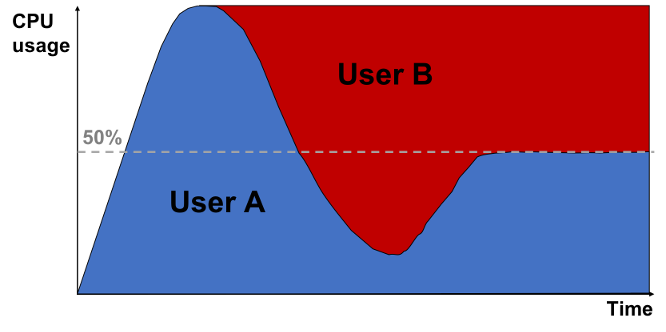
\includegraphics{images/cluster_fairshare.png}
\caption{Fairshare}
\end{figure}

    Consider two users, User A and User B, who start off with the same
priority. User A starts running some jobs and gets the full share of
available CPUs. User B now starts submitting some jobs. Initially, User
B gets a smaller proportion of CPUs than User A. As the jobs submitted
by User A start to finish, User B starts to get a larger share of the
CPUs. This is because User A now has a lower priority. Eventually, over
a period of 48 hours or so, User A and User B will have equal priorities
again and will have used an equal proportion of the cluster resources.

At Sanger we use \textbf{hierarchical fairshare} which means that the
initial priority for each user will also depend on their group
membership. This is because the system needs to accommodate the needs of
both the pipelines and the users.

Priority will only affect the decision on which jobs run next. It will
\textit{not} affect jobs that are already running. Sanger users can find
more information about fairshare
\href{mediawiki.internal.sanger.ac.uk/index.php/LSF_hierarchical_fair_share}{here}.

    You can check your priority in a particular queue using \texttt{bqueues}
and the \texttt{-r} option followed by the name of the queue that you
want to look at.

    \begin{verbatim}
bqueues -r <queue_name>
\end{verbatim}

    \begin{verbatim}
USER/GROUP   SHARES  PRIORITY  STARTED  RESERVED  CPU_TIME  RUN_TIME   ADJUST
userA           1       0.333      0        0         0.0        0       0.000
userB           1       0.211      0        0      7450.8     8924       0.000
userC           1       0.104      0        0     11218.3    34168       0.000
userD           1       0.044      0        0     72918.9   100394       0.000
userE           1       0.003     16        0    205565.6  1369196       0.000
\end{verbatim}

\newpage

    \subsection{What's next?}\label{whats-next}

For an overview of jobs arrays and dependencies, you can go back to
\href{job_arrays.ipynb}{job arrays and dependencies}. Otherwise, let's
take a look at \href{troubleshooting.ipynb}{troubleshooting}.


    % Add a bibliography block to the postdoc



\newpage






    \section{Troubleshooting}\label{troubleshooting}

    \subsection{My job failed. How do I find out what went
wrong?}\label{my-job-failed.-how-do-i-find-out-what-went-wrong}

There are many different reasons why a job might have failed. The first
place to check are the output and error files.

Let's say we submitted the wrong command, writing \texttt{slep\ 10}
instead of `sleep 10.

\begin{terminalinput}
\begin{Verbatim}[commandchars=\\\{\}]
\llap{\color{black}\LARGE\faKeyboardO\hspace{1em}} bsub \PYZhy{}o bad\PYZus{}cmd.o \PYZhy{}e bad\PYZus{}cmd.e \PY{l+s+s2}{\PYZdq{}slep 10\PYZdq{}}
\end{Verbatim}
\end{terminalinput}


    Use \texttt{bjobs} to see when your job has finished running. The jobs
status (STAT) will be \textit{EXIT}. This means that your job had an
abnormal exit and there was an issue. Below is an example.

    \begin{verbatim}
JOBID   USER    STAT  QUEUE      FROM_HOST   EXEC_HOST   JOB_NAME   SUBMIT_TIME
1000    userA   EXIT  normal     pcs5a       pcs5c       slep 10    Jan 15 10:48
\end{verbatim}

    Now, print the contents of the output file to the terminal using
\texttt{cat} (probably best to use \texttt{less} if the file is larger).

\begin{terminalinput}
\begin{Verbatim}[commandchars=\\\{\}]
\llap{\color{black}\LARGE\faKeyboardO\hspace{1em}} cat bad\PYZus{}cmd.o
\end{Verbatim}
\end{terminalinput}


    \begin{verbatim}
------------------------------------------------------------
Sender: LSF System <lsfadmin@pcs5c>
Subject: Job 4017581: <slep 10> in cluster <pcs5> Exited

Job <slep 10> was submitted from host <pcs5a> by user <userA> in cluster <pcs5>.
Job was executed on host(s) <pcs5c>, queue <normal>, user <userA> cluster <pcs5>.
</nfs/users/nfs_u/userA> was used as the home directory.
</nfs/users/nfs_u/userA> was used as the working directory.
Started at Thu Jan 15 10:48:46 2019
Results reported on Thu Jan 15 10:48:47 2019

Your job looked like:

------------------------------------------------------------
# LSBATCH: User input
slep 10
------------------------------------------------------------

Exited with exit code 127.

Resource usage summary:

    CPU time :                                   0.09 sec.
    Total Requested Memory :                     -
    Delta Memory :                               -

The output (if any) is above this job summary.



PS:

Read file <bad_cmd.e> for stderr output of this job.
\end{verbatim}

    This tells us that the job \texttt{Exited\ with\ exit\ code\ 127}. Any
exit code \textgreater{} 0 means there was an error. In this case, it
was error code 127 which means that the command we tried to run,
\texttt{slep}, could not be found.

Here is an overview of the possible exit codes:

\begin{itemize}
\tightlist
\item
  \textbf{less than 127} - there was an exit code from your script or
  command
\item
  \textbf{127} - the command was not found / doesn't exist
\item
  \textbf{more than 127} - the job was killed by a signal
\end{itemize}

When a job gets killed by a signal (error code \textgreater{} 127), you
can subtract 128 from the error code to get the signal number. You can
then run \texttt{man\ 7\ signal} to find the meaning of that signal.
Error codes 130 and 140 will typically mean you your job exceeded the
resources you requested. Try submitting the job again, requesting more
memory or to a queue with a longer time limit.

For more information about exit codes, please see the
\href{https://www.ibm.com/support/knowledgecenter/en/SSETD4_9.1.2/lsf_admin/job_exit_codes_lsf.html}{job
exit codes},
\href{https://www.ibm.com/support/knowledgecenter/en/SSETD4_9.1.2/lsf_admin/job_exception_lsf.html}{job
exception} and
\href{https://www.ibm.com/support/knowledgecenter/en/SSETD4_9.1.2/lsf_admin/job_exit_info_view_logged.html}{exit
information} sections in the LSF user guide.

    We can see the error that was generated by printing the contents of the
error file to the terminal with \texttt{cat}.

\begin{terminalinput}
\begin{Verbatim}[commandchars=\\\{\}]
\llap{\color{black}\LARGE\faKeyboardO\hspace{1em}} cat bad\PYZus{}cmd.e
\end{Verbatim}
\end{terminalinput}


    \begin{verbatim}
/tmp/1547722126.4017581: line 8: slep: command not found
\end{verbatim}

    Here we can see this confirms that the system couldn't find the command
\texttt{slep}. Whenever you have an issue with an LSF job and need to
contact your support team for help, it is always a good idea to give
them the JOBID and/or the location of the output and error files. This
makes tracking down the issue much quicker!

    \begin{center}\rule{0.5\linewidth}{\linethickness}\end{center}

    \subsection{Why can't I submit any more jobs to a particular
queue?}\label{why-cant-i-submit-any-more-jobs-to-a-particular-queue}

Some queues have limits, such as the yesterday queue, while others, like
the normal queue, have no limit. You can check the queue limits using
\texttt{bqueues}.

\begin{terminalinput}
\begin{Verbatim}[commandchars=\\\{\}]
\llap{\color{black}\LARGE\faKeyboardO\hspace{1em}} bqueues
\end{Verbatim}
\end{terminalinput}


    Each queue has a maximum number of \textbf{job slots} which can be used
by scheduled jobs in the queue. Job slots are reserved by jobs which are
pending and used by those which have already started running but are not
yet finished. In this example we can see the maximum number of job slots
for each queue by looking at the \textbf{MAX} column.

    \begin{verbatim}
QUEUE_NAME      PRIO STATUS          MAX JL/U JL/P JL/H NJOBS  PEND   RUN  SUSP
system          1000 Open:Active       -    -    -    -     0     0     0     0
yesterday       500  Open:Active      20    8    -    -     0     0     0     0
small            31  Open:Active       -    -    -    -     0     0     0     0
normal           30  Open:Active       -    -    -    -    35    13     1     0
long              3  Open:Active      50    -    -    - 31686 31636    46     0
basement          1  Open:Active      20   10    -    -   180   170    10     0
\end{verbatim}

    Sometimes there are also limits on the job slots that are available to
users. You can check this by looking at the \textbf{JL/U} column. In
this example, the yesterday queue is limited to a maximum of 8 job slots
per user and the basement to 10 job slots per user.

For more information on queues, please see \href{queues.ipynb}{queues}.

    \begin{center}\rule{0.5\linewidth}{\linethickness}\end{center}

    \subsection{I've lots of submitted jobs, how can I get my high priority
job running
first?}\label{ive-lots-of-submitted-jobs-how-can-i-get-my-high-priority-job-running-first}

There are two things that you can do to influence the order in which
your pending jobs will be run. First, you can move your job using
\textbf{\texttt{bswitch}}.

    \begin{verbatim}
JOBID   USER    STAT  QUEUE      FROM_HOST   EXEC_HOST   JOB_NAME   SUBMIT_TIME
1000    userA   PEND  normal     pcs5b                   job1       Jan 15 14:06
\end{verbatim}

    We can take a look at which queues are available using \texttt{bqueues}.

    \begin{verbatim}
QUEUE_NAME      PRIO STATUS          MAX JL/U JL/P JL/H NJOBS  PEND   RUN  SUSP
system          1000 Open:Active       -    -    -    -     0     0     0     0
yesterday       500  Open:Active      20    8    -    -     0     0     0     0
small            31  Open:Active       -    -    -    -     0     0     0     0
normal           30  Open:Active       -    -    -    -    35    13     1     0
long              3  Open:Active      50    -    -    - 31686 31636    46     0
basement          1  Open:Active      20   10    -    -   180   170    10     0
\end{verbatim}

    Look at the priorities of the queues (PRIO) to try and find a queue with
a higher priority. Here, the \textit{yesterday} queue has a higher
priority (500) compared to the normal queue (30). So, we can try moving
our job from the normal queue into the yesterday queue.

    \begin{verbatim}
bswitch 1000 yesterday
\end{verbatim}

    If we then ran \texttt{bjobs} we would see our job has been moved to the
yesterday queue.

    \begin{verbatim}
JOBID   USER    STAT  QUEUE      FROM_HOST   EXEC_HOST   JOB_NAME   SUBMIT_TIME
1000    userA   PEND  yesterday  pcs5b                   job1       Jan 15 14:06
\end{verbatim}

    Alternatively, you can use \texttt{btop} to move a pending job to the
top of your job list. In the example below, we have used \texttt{bjobs}
which showed us that we have 4 jobs scheduled: 1 running and 3 pending.

    \begin{verbatim}
JOBID   USER    STAT  QUEUE      FROM_HOST   EXEC_HOST   JOB_NAME   SUBMIT_TIME
1000    userA   RUN   normal     pcs5b       pcs5c       job1       Jan 15 14:06
1001    userA   PEND  normal     pcs5b                   job2       Jan 15 14:07
1002    userA   PEND  normal     pcs5b                   job3       Jan 15 14:08
1003    userA   PEND  normal     pcs5b                   job4       Jan 15 14:09
\end{verbatim}

    All of these jobs are identical, so \textit{job2} will be the first of our
pending jobs to be executed when the necessary resources become
available. But, what if we needed \textit{job4} to be executed first?

    \begin{verbatim}
btop 1003
\end{verbatim}

    Using \texttt{btop} followed by the JOBID will move the job (e.g. job4)
to the top of the list of jobs waiting to be executed.

    \begin{verbatim}
JOBID   USER    STAT  QUEUE      FROM_HOST   EXEC_HOST   JOB_NAME   SUBMIT_TIME
1000    userA   RUN   normal     pcs5b       pcs5c       job1       Jan 15 14:06
1003    userA   PEND  normal     pcs5b                   job4       Jan 15 14:09
1001    userA   PEND  normal     pcs5b                   job2       Jan 15 14:07
1002    userA   PEND  normal     pcs5b                   job3       Jan 15 14:08
\end{verbatim}

    For more information on job management, please see
\href{job_management.ipynb}{job management}.

    \begin{center}\rule{0.5\linewidth}{\linethickness}\end{center}

    \subsection{All of my jobs are pending. Why can't I get anything
running?}\label{all-of-my-jobs-are-pending.-why-cant-i-get-anything-running}

The first thing to do here is check how busy the cluster is using
\textbf{bqueues}.

\begin{terminalinput}
\begin{Verbatim}[commandchars=\\\{\}]
\llap{\color{black}\LARGE\faKeyboardO\hspace{1em}} bqueues
\end{Verbatim}
\end{terminalinput}


    Most commonly, your jobs will be pending because the cluster is busy and
it may just take some time for things to get running. Once other
people's jobs start to finish, resources will become available and your
jobs should start running.

If this keeps happening, there are two things to consider. The first is
whether you've requested more resources than your job is likely to
require. Let's use the \texttt{sleep} command as an example. Well
reserve 2GB (2000MB) of memory for this job.

\begin{terminalinput}
\begin{Verbatim}[commandchars=\\\{\}]
\llap{\color{black}\LARGE\faKeyboardO\hspace{1em}} bsub \PYZhy{}o sleep.o \PYZhy{}e sleep.e \PYZhy{}R \PY{l+s+s1}{\PYZsq{}select[mem\PYZgt{}2000] rusage[mem=2000]\PYZsq{}} \PY{l+s+se}{\PYZbs{}}
        \PYZhy{}M \PY{l+m}{2000} \PY{l+s+s2}{\PYZdq{}sleep 10\PYZdq{}}
\end{Verbatim}
\end{terminalinput}


    Once that has finished, take a look at the output file (sleep.o).

\begin{terminalinput}
\begin{Verbatim}[commandchars=\\\{\}]
\llap{\color{black}\LARGE\faKeyboardO\hspace{1em}} cat sleep.o
\end{Verbatim}
\end{terminalinput}


    We want to look at the amount of resources our job used.

    \begin{verbatim}
Resource usage summary:

    CPU time :                                   0.23 sec.
    Max Memory :                                 6 MB
    Average Memory :                             6.00 MB
    Total Requested Memory :                     2000.00 MB
    Delta Memory :                               1994.00 MB
    Max Swap :                                   44 MB
    Max Processes :                              3
    Max Threads :                                4
\end{verbatim}

    Here we can see that this job used only used 6MB of memory (Max Memory).
We requested 2GB (2000MB) which was 1994MB more than our job required
(Delta Memory).

You should always try to request only the resources that you need. If
you're running a large analysis, try running the analysis on a small
subset of the data and scale up to estimate the resources you'll
require.

Alternatively, it could be because your priority is low. Perhaps you or
other members of your group have been running a lot of jobs or using a
lot of resources in the last 48 hours. This can decrease your priority
and chances of getting jobs running. For more information, please see
\href{priority_and_fairshare.ipynb}{priority and fairshare}.

    \begin{center}\rule{0.5\linewidth}{\linethickness}\end{center}

    \subsection{I made a mistake when I submitted my job, can I update
it?}\label{i-made-a-mistake-when-i-submitted-my-job-can-i-update-it}

If the job is already running, it's probably best to cancel it with
\texttt{bkill}, update the command or script and then submit it again as
a new job.

    \begin{verbatim}
bkill <JOBID>
\end{verbatim}

    However, if your job is pending, you can use \textbf{\texttt{bmod}} to
update your job.

    \begin{verbatim}
bmod <options_or_command_to_update> <JOBID>
\end{verbatim}

    To update the command, you can use the \texttt{-Z} option. For example,
if we made a mistake an spelt the \texttt{sleep} command wrong and ran
\texttt{slep}:

    \begin{verbatim}
bsub "slep 60"
\end{verbatim}

    Now let's say it submitted the job, we now have a JOBID of 1000 and that
the job is pending.

    \begin{verbatim}
JOBID   USER    STAT  QUEUE      FROM_HOST   EXEC_HOST   JOB_NAME   SUBMIT_TIME
1000    userA   PEND  normal     pcs5b                   slep 60    Jan 15 14:06
\end{verbatim}

    We can update the command using \texttt{bmod} with the \texttt{-Z}
option, followed by the JOBID (1000), to update the job to run the
correct command.

    \begin{verbatim}
bmod -Z "sleep 60" 1000
\end{verbatim}

    When the job is dispatched and executed, it will now run
\texttt{sleep\ 60} instead of \texttt{slep\ 60}. You can change many
other job parameters using \texttt{bmod} such as the job name.

Let's call our job something more useful like "sleepyjob" using the
\texttt{-J} option.

    \begin{verbatim}
bmod -J sleepyjob 1000
\end{verbatim}

    We can add an output and error file too using the \texttt{-o} and
\texttt{-e} options.

    \begin{verbatim}
bmod -o sleepyjob.o -e sleepyjob.e 1000
\end{verbatim}

    Or, we can update the resources it's requesting using the \texttt{-M},
\texttt{-R} and \texttt{-n} options.

    \begin{verbatim}
bmod -n 2 -R "span[hosts=1] select[mem>2000] rusage[mem=2000]" -M 2000 1000
\end{verbatim}

    This would be updating job 1000 and asking LSF to reserve 2
cores/threads and 2GB (2000MB) memory.

    \begin{center}\rule{0.5\linewidth}{\linethickness}\end{center}

    \subsection{What's next?}\label{whats-next}

For an overview of priority and fairshare, you can go back to the
\href{priority_and_fairshare.ipynb}{priority\_and\_fairshare}.
Otherwise, you can take a look at our \href{cheat_sheet.ipynb}{LSF cheat
sheet}.


    % Add a bibliography block to the postdoc



\newpage






    \section{Cheat sheet}\label{cheat-sheet}

Below is a list of commands and their meaning taken from the LSF user
guide
\href{https://www.ibm.com/support/knowledgecenter/SSETD4_9.1.3/lsf_users_guide}{here}.

    \begin{center}\rule{0.5\linewidth}{\linethickness}\end{center}

    \subsection{Cluster overview}\label{cluster-overview}

\begin{itemize}
\item
  \textbf{lshosts} - Displays information about hosts in the cluster
\item
  \textbf{bhosts} - Displays information about hosts and their resources
\item
  \textbf{lsid} - Displays the cluster name
\item
  \textbf{lsclusters} - Displays cluster status and size
\end{itemize}

    \begin{center}\rule{0.5\linewidth}{\linethickness}\end{center}

    \subsection{Queue information}\label{queue-information}

\begin{itemize}
\tightlist
\item
  \textbf{bqueues} - Displays information about queues
\end{itemize}

    \begin{center}\rule{0.5\linewidth}{\linethickness}\end{center}

    \subsection{Job execution management}\label{job-execution-management}

\begin{itemize}
\item
  \textbf{bjobs} - Displays information about scheduled jobs
\item
  \textbf{bsub} - Submits job(s) for execution
\item
  \textbf{bstop} - Suspends job(s)
\item
  \textbf{bresume} - Resumes suspended job(s)
\item
  \textbf{bkill} - Cancels scheduled job(s)
\item
  \textbf{bswitch} - Moves job(s) to a different queue
\item
  \textbf{bmod} - Modifies the properties of pending job(s)
\item
  \textbf{btop} - Moves job(s) relative to your first job in the queue
\item
  \textbf{bbot} - Moves job(s) relative to your last job in the queue
\end{itemize}

    \begin{center}\rule{0.5\linewidth}{\linethickness}\end{center}

    \subsection{General information}\label{general-information}

\begin{itemize}
\tightlist
\item
  \textbf{bacct} - Displays accounting statistics about finished jobs
\end{itemize}

    \begin{center}\rule{0.5\linewidth}{\linethickness}\end{center}

    \subsection{bqueues}\label{bqueues}

Get more information about a particular queue:

\begin{verbatim}
bqueues -r <queue_name>
\end{verbatim}

    \begin{center}\rule{0.5\linewidth}{\linethickness}\end{center}

    \subsection{bsub}\label{bsub}

Submit a job:

\begin{verbatim}
bsub <command>
\end{verbatim}

Submit a job to a particular queue:

\begin{verbatim}
bsub -q <queue_name> <command>
\end{verbatim}

Submit a job which writes output and errors to file:

\begin{verbatim}
bsub -o <output_file> -e <error_file> <command>
\end{verbatim}

Submit a job reserving 1GB (1000MB) memory:

\begin{verbatim}
bsub -M 1000 -R 'select[mem>1000] rusage[mem=1000]' <command>
\end{verbatim}

Submit a job requiring 8 threads:

\begin{verbatim}
bsub -n 8 <command>
\end{verbatim}

    \begin{center}\rule{0.5\linewidth}{\linethickness}\end{center}

    \subsection{bjobs}\label{bjobs}

List jobs owned by all users:

\begin{verbatim}
bjobs -u all
\end{verbatim}

List jobs owned by a particular user:

\begin{verbatim}
bjobs -u <username>
\end{verbatim}

List jobs for all users in a particular queue:

\begin{verbatim}
bjobs -u all -q <queue_name>
\end{verbatim}

List your pending jobs:

\begin{verbatim}
bjobs -p
\end{verbatim}

List your running jobs:

\begin{verbatim}
bjobs -r
\end{verbatim}

List your finished jobs:

\begin{verbatim}
bjobs -d
\end{verbatim}

List your suspended jobs:

\begin{verbatim}
bjobs -s
\end{verbatim}

Get more information about a particular job:

\begin{verbatim}
bjobs -l <JOBID>
\end{verbatim}

    \begin{center}\rule{0.5\linewidth}{\linethickness}\end{center}

    \subsection{bstop}\label{bstop}

Suspend a job:

\begin{verbatim}
bstop <JOBID>
\end{verbatim}

    \begin{center}\rule{0.5\linewidth}{\linethickness}\end{center}

    \subsection{bresume}\label{bresume}

Resume a job:

\begin{verbatim}
bresume <JOBID>
\end{verbatim}

    \begin{center}\rule{0.5\linewidth}{\linethickness}\end{center}

    \subsection{bkill}\label{bkill}

Cancel a job:

\begin{verbatim}
bkill <JOBID>
\end{verbatim}

    \begin{center}\rule{0.5\linewidth}{\linethickness}\end{center}

    \subsection{bswitch}\label{bswitch}

Move job to a different queue:

\begin{verbatim}
bswitch <destination_queue> <JOBID>
\end{verbatim}

    \begin{center}\rule{0.5\linewidth}{\linethickness}\end{center}

    \subsection{bmod}\label{bmod}

Modify the parameters of a pending job:

\begin{verbatim}
bmod <options> <JOBID>
\end{verbatim}

Update the job name:

\begin{verbatim}
bmod -J <new_job_name> <JOBID>
\end{verbatim}

Update the output and error file paths:

\begin{verbatim}
bmod -o <output_file> -e <error_file> <JOBID>
\end{verbatim}

Update the job resources:

\begin{verbatim}
bmod -M <memory_in_MB> -R 'select[mem><memory_in_MB>] rusage[mem=<memory_in_MB>]' <JOBID>
\end{verbatim}

    \begin{center}\rule{0.5\linewidth}{\linethickness}\end{center}

    \subsection{btop}\label{btop}

Move job to the top of your job list:

\begin{verbatim}
btop <JOBID>
\end{verbatim}

    \begin{center}\rule{0.5\linewidth}{\linethickness}\end{center}

    \subsection{bbot}\label{bbot}

Move job to the bottom of your job list:

\begin{verbatim}
bbot <JOBID>
\end{verbatim}


    % Add a bibliography block to the postdoc



\end{document}
